
    The research contributions of this thesis are based on a novel constraint
    programming approach on Static Single Assignment (SSA) compiler intermediate
    representation.
    This chapter derives and motivates the underlying methodology, which is
    then used as the basis for
    \Cref{chapter:candl,chapter:reductions,chapter:idioms}.
    The constraint programming approach is derived in three steps.

    First, an overview of program representations during different compilation
    stages is given, and the particular features of SSA representations are
    highlighted.
    These features are then used to derive a model that captures the static
    structure of SSA programs.
    The section uses some mathematical notation in an attempt to build a
    reliable foundation for later parts of the thesis.
    The {\it List of Symbols and Notation} contains many of the presumed
    notational conventions.
    The SSA model is initially derived generically and then demonstrated in
    more detail on \mbox{LLVM IR}, a specific SSA compiler intermediate
    representation.

    After the derivation of the SSA model, the concept of SSA constraint
    problems is defined.
    These are formulas that impose restrictions on parts of SSA code,
    formulated as constraints on the SSA model.
    SSA constraint problems define code structures such as loops, and detecting
    adhering code sections in SSA code is then equivalent to finding
    solutions to the constraints.
    The structure of several classes of constraint formulas is discussed,
    reflecting conventional compiler analysis methods like data flow,
    dominance relationships, and data type restrictions.

    Finally, efficient algorithms for SSA solving constraint problems are
    derived.
    Backtracking is used to find solutions quickly by incrementally extending
    partial solutions.
    The structure of specific classes of SSA constraint problems is analysed,
    and efficient backtracking solutions are derived individually, yielding
    composable building blocks for the solver.
    After deriving the algorithms, implementation considerations are
    discussed.
    Suitable data structures are selected, and runtime complexity is analysed.
    To conclude the chapter, similarities and differences to standard
    Satisfiability Modulo Theory (SMT) problems are explored.

%    Constraint formulas on SSA respresentations initially appear to mimic
%    pattern matching approaches on abstract syntax tree (AST) level.
%    However, they quickly prove themselves to be vastly more expressive.
%    Some consideration is necessary to handle search space explosion, but
%    the reward are much more powerful recognition capabilities and the
%    expression of higher level algorithmic structures, which are impossible to
%    define syntactically on programming language level.
%    Later chapters will explore the power of this approach in detail, by
%    building a complete constraint programming language on top of the theory in
%    this chapter, and by then using it to solve real compiler analysis problems.

%    After defining a mathematical foundation of SSA form and introducing
%    formalisms for the expression of basic constraint problems on top of it,
%    several standard definitions from compiler theory are reformulated in the
%    framework.
%    This includes common graph properties, including the concept of domination,
%    as well as control flow structures such as single entry single exit blocks.
%    All of this lays the foundations for the succeeding chapter.

%    Finally, for the practical application of constraint programming to compiler
%    intermediate representation, efficient solver techniques are needed.
%    The last section in this chapter discusses strategies for limiting
%    compile time explosion and explores analogies of the described model to
%    standard Satisfiability Modulo Theory (SMT) problems.
%    This gives further insights into performance improvements and puts the
%    work into a broader theoretical context.

\section{Introduction}

    Modern compilers for procedural languages such as
    C/C++, Fortran or JavaScript typically use a succession of different
    representations for the program during compilation.
    They reflect the requirements of the compilation stages in which they are
    used.

    \begin{description}[style=unboxed,leftmargin=0cm,labelindent=\parindent]
    \item[Front end representations] are close to the source program and
    are strongly influenced by the specific grammar of the programming language.
    Typically, they are built around an abstract syntax tree with additional
    annotations, such as type information.
    These representations are rich in information about syntactic and stylistic
    choices of the programmer, and they scale in complexity with the source
    language.
    Some advanced language features, such as overloaded operators, are not
    resolved in this class of representations.
    Therefore, the semantics of program parts in these representations
    is highly dependent on context.

    \item[\bf Back end representations] are based on a model of the target
    hardware.
    They typically approach an assembly style format and expose the instruction
    set architecture of the hardware, making them platform-specific.
    Back end representations also encode decisions for problems that are removed
    from the algorithmic content of the user program, such as instruction
    selection and register allocation.

    \item[\bf Middle end representations] are designed to enable the analysis
    and transformation of code in order to apply optimisations.
    {\bf Static Single Assignment} (SSA) representations have emerged as a
    common choice for the middle end in leading compilers.
    SSA abstracts away the complexities of the source language and the
    target architecture, focusing on a relatively simple description of the
    semantics of the user program.
    This enables reliable analysis and platform-independent reasoning.
    \end{description}

    Static Single Assignment was first proposed by
    \citet{Rosen:1988:GVN:73560.73562}, and there are now many different
    compiler intermediate representations that implement the concept.
    Instruction set, type system and syntax
    (if a textual representation is even specified) of these representations
    vary considerably, depending on the requirements of the source languages
    (static or dynamic) and the operating constraints
    (just-in-time or ahead-of-time).
    Some prominent examples of compilers using SSA include
    {\bf clang} (LLVM IR), {\bf GCC} (GIMPLE), {\bf v8 Crankshaft} (Hydrogen),
    and {\bf SpiderMonkey} (IonMonkey/MIR).
    Despite many differences, they share the same basic structure that is
    discussed in this chapter.

    SSA form was developed as an improvement over previously used
    compiler intermediate representations.
    Specifically, the eponymous static single assignment property applies to
    more general {\em linear intermediate representations} as an additional
    restriction, as described in \citet{Torczon:2007:EC:1526330}.
    The following \Cref{sec:ssaf} gives an overview of the characteristic shared
    features of SSA representations that are relevant for this work.

\subsection{Static Single Assignment Form}
\label{sec:ssaf}

    SSA representations are linear intermediate representations, meaning that
    they represent each function as a single linear sequence of instructions.
    These instructions operate on an unlimited amount of registers, using a well
    defined -- but representation specific -- instruction set.
    Branch instructions are used to redirect the execution conditionally or
    unconditionally.
    Consecutive instructions with no branching between them are grouped into
    basic blocks.
    Within these, instructions are executed in order of appearance.
    Basic blocks may have labels or be identified simply by enumerating them.
    Instruction arguments can be registers, constants, globals or function
    parameters.
    Branch instructions furthermore take basic block arguments as branch
    targets.
    Instructions may write their result into a single output register.

    The SSA property stipulates that within a function, no register can be
    written at more than a single static location.
    This means that registers can be identified directly with the instructions
    that define them.
    The registers can, therefore, be made implicit, with only the data flow
    between instructions required to recover them.
    In the presence of dynamic control flow, \mbox{$\Phi$-instructions} are
    required to uphold the SSA property.
    These \mbox{$\Phi$-instructions} are placed at the beginning of a basic
    block, and select one of several values dynamically, depending on the origin
    of incoming branches, i.e.\ depending on the previously visited
    basic block.

    \Cref{fig:ssaoverview} shows how SSA programs can be represented as a
    hierarchy of lists.
    Programs are lists of functions, which are lists of basic blocks, which are
    lists of instructions, which take lists of arguments.
    The ability to enumerate all these entities in linear sequences enables the
    identification of integers with SSA values in the later sections of this
    chapter.

\begin{figure}[h]
\centering
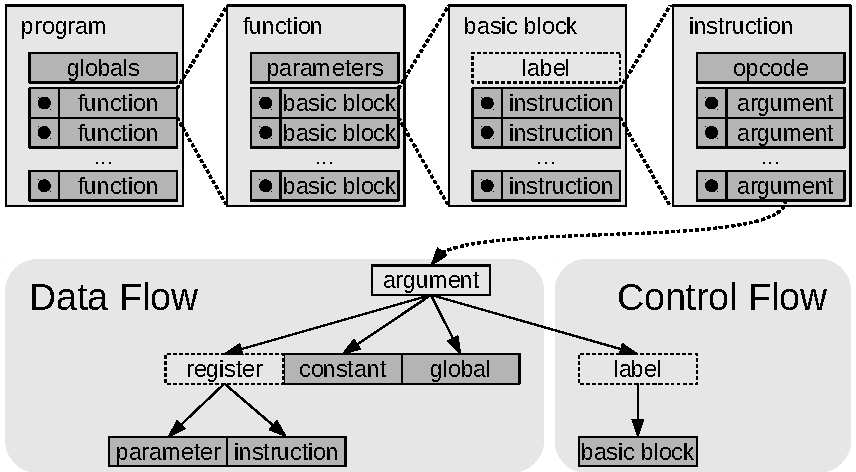
\includegraphics[width=\textwidth]{figures/ssaoverview}
\caption{Structural overview of SSA: Programs are represented as hierarchies of
    lists. The SSA property makes registers implicit; values can be statically
    matched to defining instructions.}
\label{fig:ssaoverview}
\end{figure}

\subsection{The Emergence of Static Single Assignment Form}

    \Cref{ssaexample} shows how critical features of SSA form emerge from
    simplification steps of source code.
    This is demonstrated on the ``{\tt sqrt}'' example function that
    approximates the square root of a double-precision floating-point value
    in C, using the Babylonian method described in \Cref{babylonian_equation}.

\begin{equation}
    x_0\approx\sqrt{S},\text{\hspace{1cm}}
    x_{n+1}=\frac{x_n+\frac{S}{x_n}}{2}\text{\hspace{1cm}}
    \implies\text{\hspace{1cm}}
    \lim_{n\rightarrow\infty}x_n=\sqrt{S}
    \label{babylonian_equation}
\end{equation}

    Starting from the source code {\bf(a)} at the top left of the figure, the
    function is first modified by breaking down complex expressions.
    The expressions are turned into sequences of basic operations, shown at the
    top right {\bf(b)}.
    Explicit variables appear for the previously implicit temporary values.
    This simplifies the program, with many of the operations directly mapping to
    individual processor instructions.
    Furthermore, different input programs get mapped to the same,
    predictable output by this transformation, making it a normalisation.

    In a second step, the structured control flow of the program is replaced
    with goto statements that coordinate the control flow between basic blocks.
    This is shown at the bottom right {\bf(c)}.
    While this does not ease the intuitive understanding of the program, it
    unifies several distinct control flow structures provided in the source
    language into a single mechanism.
    This simplifies program analysis.
    Importantly, no relevant information is lost by discarding the control flow
    structures.
    They can be reconstructed algorithmically.

    Finally, the Static Single Assignment property is introduced at the bottom
    left {\bf(d)}.
    Each variable that is assigned in more than one static locations in the
    program is instead duplicated into multiple variables.
    Where necessary, these now distinct variables are bound together with
    $\Phi$-instructions.
    This cannot be expressed in the C programming language syntax.
    Instead, the behaviour is documented by comments in lines 8--13.

    The impact of the SSA property seems minor at first, but convenient
    implications can be identified already within the C language.
    As all local variables are written in exactly one static location, each
    variable can be declared and defined in the same place.
    This means that it is always known statically, which expression yielded the
    value of each variable.
    This immediately guarantees that the variable ``\texttt{i}'' in the example
    always has the value \texttt{0}, and that the variable~``\texttt{x}'' always
    has the value \texttt{1.0}.

    This section developed an understanding of how SSA form originated
    historically and how it emerges during the compilation process.
    The following section uses the observations from
    \Cref{fig:ssaoverview} -- that most parts of SSA code can be enumerated
    and represented as elements in lists -- to derive a model of the static
    structure of SSA programs.
    This model then serves as the foundation of later sections, which define
    compiler analysis problems via constraint formulas on this model.

\begin{figure}[p]
    \begin{minipage}{0.48\textwidth}
\begin{lstlisting}[language=C,captionpos=t,title=
   {{\bf(a)} {} C source function:\leftskip=0pt}]
double sqrt(double S) {
  double x = 1.0;
  for(int i=0; i<N; i+=1)
    x = 0.5 * (x + S / x);
  return x;
}
\end{lstlisting}
\begin{lstlisting}[language=C,captionpos=t,title=
   {{\bf(d)} {} The SSA property is introduced:\leftskip=0pt}]
double sqrt(double S) {
entry:
  double x = 1.0;
  int i = 0;
  goto header;

header:
  int i2 = /* if reached
    from line  5: i,
    from line 23: i3 */
  int x2 = /* if reached
    from line  5: x,
    from line 23: x3 */
  bool test = i2 < N;
  if(test) goto loop;
      else goto exit;

loop:
  double t1 = S / x2;
  double t2 = x2 + t1;
  double x3 = 0.5 * t2;
  int i3 = i2+1;
  goto header;

exit:
    return x2;
}
\end{lstlisting}
\end{minipage}
\hfill
\begin{minipage}{0.48\textwidth}
\begin{lstlisting}[language=C,basicstyle=\linespread{1.06451612903}\ttfamily,
                   captionpos=t,title=
   {{\bf(b)} {} Complex expressions are broken down:\leftskip=0pt}]
double sqrt(double S) {
  double x = 1.0;
  for(int i=0; i<N; i+=1)
  {
    double t1 = S / x;
    double t2 = x + t1;
    x = 0.5 * t2;
  }
  return x;
}
\end{lstlisting}
\begin{lstlisting}[language=C,basicstyle=\linespread{1.06451612903}\ttfamily,
                   captionpos=t,title=
   {{\bf(c)} {} Structured control flow is expanded:\leftskip=0pt}]
double sqrt(double S) {
entry:
  double x = 1.0;
  int i = 0;
  goto header;

header:
  bool test = i < N;
  if(test) goto loop;
      else goto exit;

loop:
  double t1 = S / x;
  double t2 = x + t1;
  x = 0.5 * t2;
  i = i+1;
  goto header;

exit:
    return x;
}
\end{lstlisting}
\end{minipage}

    \caption{Static Single Assignment emerges from successive simplification
             and normalisation of source language features: 
             Demonstration on an example C function that approximates the
             square root of an input value with the Babylonian method.
             The transformation results {\bf (b-d)} are rendered in C.
             Real compilers typically operate on
             dedicated internal representations instead.
             \parfillskip=0pt}
    \label{ssaexample}
\end{figure}

\section{Deriving an SSA Model}
\label{sec:derivingamodel}

    This section develops a mathematical model for programs that are in
    SSA form.
    The aim is not to introduce an operational semantics of such programs, or
    more generally to derive a model for their execution.
    Instead, the section focuses on precise notation to express the static
    structure of existing SSA intermediate representations.
    The completed model will enable the generation of a program that is
    semantically equivalent to the one from which the model was extracted.
    The remainder of this section adheres to the naming conventions in
    \Cref{def:ssa}.

\begin{figure}[h]
\begin{definition}{Features of Static Single Assignment Functions}{ssa}
    For the remainder of this section, some function $\mathcal F$ in SSA form is
    assumed fixed. 
    The following identifiers are then used to describe the features of this
    function.

    \begin{itemize}
    \item $|par|$ is the number of function parameters
          $par_1,\dots par_{|par|}$.
    \item $|ins|$ is the number of instructions $ins_1,\dots ins_{|ins|}$ that
          make up the function, in depth-first order, starting from the
          execution entry.
    \item $|glb|$ is the number of unique globals $glb_1,\dots glb_{|glb|}$ that
          are used as an operand of any of the instructions.
    \item $|cst|$ is the number of unique constants $cst_1,\dots cst_{|cst|}$
          that are used as an operand of any of the instructions.
    \end{itemize}
\end{definition}
\end{figure}

    This notation already implies several decisions about the SSA model that is
    derived in this section.
    Firstly, the model captures only a single function at once.
    Secondly, basic blocks are not explicitly encoded.
    Instead, all instructions of the function are enumerated sequentially in
    depth-first order, starting from the function entry.
    Basic blocks can, however, be reconstructed from the control flow, as
    discussed in \Cref{sec:remainingstructure}.
    Thirdly, the argument structure of the instructions is modelled separately.

\subsection{Data Flow and Control Flow}

    The data flow between instructions, as well as the control flow, is captured
    in graph structures.
    The Static Single Assignment property makes registers implicit, and the
    direct interaction between instructions becomes the natural model for data
    flow.
    Instruction arguments fall into four categories: function parameters,
    other instructions, constants, and globals.
    Branching instructions also take basic block labels as branch targets,
    but those are treated separately in the control flow graph that is
    introduced later.
    All instruction arguments are therefore taken from the named sets introduced
    in \Cref{def:ssa}.

    For each function, the sequences $par$, $ins$, $gbl$, $cst$ can be
    statically determined.
    Therefore, individual instruction arguments can be encoded by one integer
    each, indexing into the union of those four sequences.
%    Therefore, a single integer is enough to encode each instruction argument as
%    an index into the union of those four sequences.
    This allows for the entire argument structure of the instructions in an SSA
    function to be turned into a labelled multigraph, with edge labels
    accounting for the positional order of the arguments.
    These observations lead to the definition of the {\it set of used values} in
    \Cref{def:usedvalues} and the {\it data flow graph} in \Cref{def:dfg}.

\begin{figure}[h]
\begin{definition}{Set of Used Values}{usedvalues}
    The {\em set of used values} of the SSA function $\mathcal F$ is the tuple
    \begin{align*}
       val_1,\dots,val_{|val|} = par_1,\dots,par_{|par|},
                                 ins_1,\dots,ins_{|ins|},
                                 glb_1,\dots,glb_{|glb|},
                                 cst_1,\dots,cst_{|cst|}.
    \end{align*}
\end{definition}

\begin{definition}{Data Flow Graph}{dfg}
    The {\em data flow graph} of the SSA function $\mathcal F$ is the set
    $DFG_{\mathcal F}\subset \mathbb N^3$ such that
    \begin{align*}
        (n,a,b)\in DFG_{\mathcal F}\iff{}&1\leq a\leq |val|
            \mathrel{\land}1\leq b-|par|\leq |ins|\\
            \mathrel{\land}{}&(val_a\text{ is the $n$th argument of }ins_{b-|par|}).
    \end{align*}
    For $\Phi$-instructions, the incoming basic blocks are ordered according to
    the order on $ins$.
    The $n$th argument is the incoming value attached to the $n$th incoming
    basic blocks.
\end{definition}
\end{figure}

    Complementing the data flow graph is the control flow graph of the function,
    as introduced in \Cref{def:cfg}.
    The control flow graph is often defined with edges between basic blocks.
    However, in this definition, the edges are directly between instructions.
    This is convenient in later
    \Cref{sec:constraintprogramming,sec:constraintsolving}, where both graphs
    can be treated identically.

    The defining equation can be separated into several parts.
    The first line expresses that edges in the control flow graph are always
    between two instructions.
    The remainder of the equation gives two options, corresponding to different
    types of edges in the control flow graph.
    Firstly, there are the trivial edges within a basic block.
    Secondly, there are edges between basic blocks.


\begin{figure}[h]
\begin{definition}{Control Flow Graph}{cfg}
    The {\em control flow graph} of the SSA function $\mathcal F$ is the set
    $CFG_{\mathcal F}\subset \mathbb N^3$ such that
    \begin{align*}
        (n,a,b)&{}\in CFG_{\mathcal F}\iff 1<a-|par|\leq|ins|\mathrel{\land}1<b-|par|\leq|ins|\mathrel{\land}\\
               &\left(\begin{aligned}[c]
                                    (\neg (ins_{a-|par|}\text{ terminates basic block})\mathrel{\land}{}&b=a+1\mathrel{\land}n=1)\\
                      \mathrel{\lor}(\phantom{\neg}(ins_{a-|par|}\text{ terminates basic block})\mathrel{\land}{}&ins_{b-|par|}\text{ first instruction in}\text{ $n$th}\\[-0.5em]
                                                   &\text{target basic block of }ins_{a-|par|})
        \end{aligned}\right).
    \end{align*}
\end{definition}
\end{figure}

\subsection{Identifying Remaining Structure}
\label{sec:remainingstructure}

    \Cref{sec:derivingamodel} introduced structures to model the control flow
    and data flow of SSA programs.
    This section identifies the remaining information that the SSA model needs
    in order to capture the program semantics fully.
    This is achieved when it is possible to recreate a semantically equivalent
    program in the source SSA compiler intermediate representation from the
    model.
    Most of the program structure can already be recovered from $DFG_\mathcal F$
    and $CFG_\mathcal F$:

\begin{enumerate}
    \item The basic block boundaries are reconstructed by identifying all
          consecutive instructions $A$, $B$ where at least one of the
    conditions hold:
    \begin{itemize}
        \item $A$ does not have exactly one outgoing edge to $B$ or
        \item $B$ does not have exactly one incoming edge from $A$.
    \end{itemize}
    \item Basic block labels and register names carry no meaning and can be
          chosen arbitrarily.
    \item The arguments of all instructions can be immediately filled in from 
          $DFG_\mathcal F$.
          Similarly, $CFG_\mathcal F$ directly provides the target instructions
          for all goto statements.
    \item The positional arguments of $\Phi$-instructions in $DFG_\mathcal F$
          are attached as incoming values to the incoming basic blocks
          after ordering those according to the order on $ins$.
          The original positional order of the incoming pairs is
          not recovered, but it carries no meaning.
\end{enumerate}

    The only part of the SSA representation that still needs modelling is
    per-value information.
    This includes the opcodes of instructions, the values of constants,
    and type information.
    This is demonstrated in \Cref{fig:separation}.
    At the top of the figure is a simple function in an abstract SSA
    representation, which calculates an approximation of the square root of a
    number using the Babylonian method.
    It has 11 instructions separated into four basic blocks, with the majority
    of the instructions in a loop that iteratively improves the result.
    The entire semantic information that is encoded in this SSA representation
    can be recovered from the structures at the bottom of the figure:
    per-instruction opcode information, lists of the parameters, constants and
    globals used, the data flow graph as in \Cref{def:dfg} and the control
    flow graph as in \Cref{def:cfg}.

    Instruction sets and type systems differ between SSA representations,
    although they overlap significantly.
    This chapter aims to capture commonalities of SSA representations, the study
    of instruction sets and type systems is orthogonal to this.
    Therefore, these structures  are modelled as obaque sets as in
    \Cref{def:isatypes}.

\begin{figure}[h]
\begin{definition}{Representation Specific Sets}{isatypes}
    $Opcodes_L$ is the set of all opcodes available in the SSA language $L$,
    $Types_L$ is the set of all types in $L$,
    and $GlobalNames_L$ is the set of all available names for global values.
\end{definition}
\end{figure}

\begin{figure}[p]
\centering
\begin{minipage}{0.42\textwidth}
\begin{tabular}{|cl|}
\multicolumn{2}{c}{{\bf function} Sqrt($S$)}\\
\hline
{\bf entry} & $\text{goto } header$\\
\hline
\multirow{4}{*}{\bf header} & $i \leftarrow \Phi(entry:0,loop:i')$\\
                            & $x \leftarrow \Phi(entry:1,loop:x')$\\
                            & $c \leftarrow i<N$\\
                            & $\text{if }c\text{ goto }loop\text{ else }exit$\\
\hline
\multirow{5}{*}{\bf loop} & $t_1\leftarrow S/x$\\
                          & $t_2\leftarrow x+t_1$\\
                          & $x'\leftarrow t_2/2$\\
                          & $i'\leftarrow i+1$\\
                          & $\text{goto }header$\\
\hline
{\bf exit} & $\text{return }x$\\
\hline
\end{tabular}
\end{minipage}

\vspace{3.2mm}
{\huge
$\cong$}
\vspace{3.2mm}

$\left(
\begin{minipage}{5.5cm}
\centering
\hspace{-2em}
\begin{tabular}{r}
\phantom{00}\\
1:
\end{tabular}
\begin{tabular}{|l|}
\multicolumn{1}{p{3cm}}{{\bf parameters:}}\\
\hline
$S$\\
\hline
\end{tabular}\\
\hspace{-2em}
\begin{tabular}{r}
\phantom{88}\\
2:\\
3:\\
4:\\
5:\\
6:\\
7:\\
8:\\
9:\\
10:\\
11:\\
12:
\end{tabular}
\begin{tabular}{|l|}
\multicolumn{1}{p{3cm}}{{\bf instructions:}}\\
\hline
$\text{goto } \square$\\
$\Phi(\square:\square,\square:\square)$\\
$\Phi(\square:\square,\square:\square)$\\
$\square<\square$\\
$\text{if }\square\text{ goto }\square\text{ else }\square$\\
$\square/\square$\\
$\square+\square$\\
$\square/\square$\\
$\square+\square$\\
$\text{goto } \square$\\
$\text{return }\square$\\
\hline
\end{tabular}\\
\hspace{-2em}
\begin{tabular}{r}
\phantom{88}\\
13:
\end{tabular}
\begin{tabular}{|l|}
\multicolumn{1}{p{3cm}}{{\bf globals:}}\\
\hline
$N$\\
\hline
\end{tabular}\\
\hspace{-2em}
\begin{tabular}{r}
\phantom{88}\\
14:\\
15:\\
16:
\end{tabular}
\begin{tabular}{|l|}
\multicolumn{1}{p{3cm}}{{\bf constants:}}\\
\hline
$1$\\
$2$\\
$0$\\
\hline
\end{tabular}
\end{minipage}
\right)\hspace{1em}\text{\huge +}\hspace{1em}\left(
\begin{minipage}{5.5cm}
\centering
\setlength{\abovedisplayskip}{0pt}
\setlength{\belowdisplayskip}{0pt}
\vspace{-0.5em}
\begin{align*}
DFG_\mathcal F=\{
&10\xrightarrow{2}3,\ 16\xrightarrow{1}3,\\[-0.153em]
&9\xrightarrow{2}4,\ 14\xrightarrow{1}4,\\[-0.153em]
&3\xrightarrow{1}5,\ 13\xrightarrow{2}5,\\[-0.153em]
&5\xrightarrow{1}6\\[-0.153em]
&1\xrightarrow{1}7,\ 4\xrightarrow{2}7,\\[-0.153em]
&4\xrightarrow{1}8,\ 7\xrightarrow{2}8\\[-0.153em]
&8\xrightarrow{1}9,\ 15\xrightarrow{2}9\\[-0.153em]
&3\xrightarrow{1}10,\ 14\xrightarrow{2}10,\\[-0.153em]
&4\xrightarrow{1}12\}\\
CFG_\mathcal F=\{
&2\xrightarrow{1}3,\\[-0.153em]
&3\xrightarrow{1}4,\\[-0.153em]
&4\xrightarrow{1}5,\\[-0.153em]
&5\xrightarrow{1}6,\\[-0.153em]
&6\xrightarrow{1}7,\ 6\xrightarrow{2}12,\\[-0.153em]
&7\xrightarrow{1}8,\\[-0.153em]
&8\xrightarrow{1}9,\\[-0.153em]
&9\xrightarrow{1}10,\\[-0.153em]
&10\xrightarrow{1}11,\\[-0.153em]
&11\xrightarrow{1}3\}
\end{align*}
\end{minipage}
\right)$

\caption{SSA representation is decomposed into individual instructions, data
         flow and control flow.
         This is an equivalent representation of the function; no semantic
         information is lost.
         The example is a rendering of the Babylonian method in
         \Cref{ssaexample}, abstracting away the C syntax.
         \parfillskip=0pt}
\label{fig:separation}
\end{figure}

\subsection{Putting the Model Together}

\begin{figure}[p]
    \begin{definition}{Mathematical Model of SSA programs}{ssamodel}
    The {\em SSA model} of the function $\mathcal F$ is the tuple
    \begin{align*}
        (DFG_\mathcal{F},
         CFG_\mathcal{F},
         T_\mathcal{F},
         P_\mathcal{F},
         I_\mathcal{F},
         G_\mathcal{F},
         C_\mathcal{F}),
    \end{align*}
    where

    \begin{itemize}
    \item $DFG_\mathcal{F}\subset\mathbb N^3$ and
          $CFG_\mathcal{F}\subset\mathbb N^3$ are the data flow and control
          flow graph.
    \item $T_\mathcal F\subset\mathbb N\times Types$ is the type model, defined
          by the property
          \begin{align*}
              (k,ty)\in T_\mathcal F\iff 1\leq k\leq n_{pigc}
                  \mathrel{\land}(val_k\text{ has type }ty).
          \end{align*}
    \item $P_\mathcal F\subset\mathbb N$ and $G_\mathcal F\subset\mathbb N$
          are the parameter model and global model, defined by the properties
          \begin{align*}
              k\in P_\mathcal F\iff& 1\leq k\leq n_p\text{ and}\\
              k\in G_\mathcal F\iff& n_p+n_i<k\leq n_p+n_i+n_g.
          \end{align*}
    \item $I_\mathcal F\subset\mathbb N\times Opcodes$ is the instruction model,
          defined by the property
          \begin{align*}
              (k,op)\in I_\mathcal F\iff n_p<k\leq n_p+n_i
                  \mathrel{\land}(ins_{k-n_p}\text{ has opcode }op).
          \end{align*}
    \item $C_\mathcal F\subset\mathbb N\times\mathbb R$ is the constant model,
          defined by the property
          \begin{align*}
              (k,x)\in C_\mathcal F\iff{}&n_p+n_i+n_g<k\leq n_{pigc}\\
                        \mathrel{\land}{}&(cst_{k-n_p-n_i-n_g}
                        \text{ has numeric value equal to }x).
          \end{align*}
    \end{itemize}
\end{definition}

\begin{notation}{Graph Projections}{convenience}
    For $G\subset\mathbb N^3, k\in\mathbb N$, the following notation applies:
    \begin{align*}
        G^k:=&\{(a,b)\in\mathbb N^2\mid (a,b,k)\in G\}\\
        G^*:=&\{(a,b)\in\mathbb N^2\mid \exists c\in\mathbb N:(a,b,c)\in G\}.
    \end{align*}

    For $G\subset\mathbb N\times\mathbb R, c\in\mathbb R$, the following
    notation applies:
    \begin{align*}
        G^c:=&\{a\in\mathbb N\mid (a,c)\in G\}\\
        G^*:=&\{a\in\mathbb N\mid \exists c\in\mathbb R:(a,c)\in G\}.
    \end{align*}
\end{notation}
\end{figure}

    With separate mathematical structures in place to capture all the relevant
    information contained in SSA programs, the SSA model can now be assembled.
    \Cref{def:ssamodel} shows this completed model.
    The data flow graph $DFG_\mathcal F$ and the control flow graph
    $CFG_\mathcal F$ were discussed in detail previously, but some
    clarifications are required for the remaining structures.

    The {\it instruction model}, {\it type model}, and {\it constant model}
    assign additional information from different domains to the used values in
    the program.
    Instead of attaching one opcode to each instruction, the
    {\it instruction model} allows instructions to be linked with several
    elements in the set {\it Opcodes}.
    This is convenient to model opcode categories, where an instruction might be
    an ``arithmetic'' operation and a ``subtraction'' in particular.
    The same is true for the {\it type model}, which enables it to express
    subtyping, e.g.\ an ``integer pointer'' value can also be a ``pointer''.
    The {\it type model} can also be used to capture additional data, such as
    compiler-specific attributes and aliasing information.
    
    Finally, the {\it parameter model} and {\it global model} are encoding which
    elements in the set of used values of $\mathcal F$ are parameters and
    globals, respectively.
    Parameter names are not significant, because their positionality
    already identifies parameters uniquely within the function signature.
    Therefore, the {\it parameter model} identifies all parameters, but attaches
    no additional data.
    For global values, on the other hand, the names are attached by the
    {\it global model} as elements from the set $GlobalNames$.

\subsection{Additional Notation}

    The seven individual components of the SSA model are each expressed as a
    set of tuples.
    In order to conveniently manipulate these structures, 
    \Cref{def:convenience} introduces several functions and shorthand notation.

    For a set of tuples, the function $head$ returns the set of all the first
    elements of the tuples.
    For example, $head(I_\mathcal F)$ yields all the opcodes that are used in
    the function $\mathcal F$.
    Correspondingly, the function $tails$ removes the first element of all
    tuples within a set.
    For example, $tails(I_\mathcal F)$ identifies the indices of all the
    instructions within the set of used values of $\mathcal F$, but removes the
    information about their opcodes.
    Finally, the $select$ function is used to filter a set for only those tuples
    with a specific first element, and then returns the tails of all these
    tuples.
    For example, $select(add,I_\mathcal F)$ gives the indices of all $add$
    instructions within the set of used values of the function $\mathcal F$.

    The representation of data flow and control flow using labelled multigraphs
    contains more information than is required for some tasks.
    The simplified versions $DFG_\mathcal F^*$ and $CFG_\mathcal F^*$ are
    constructed with the $tails$ function, effectively removing the labels and
    resulting in ordinary graph structures.
    Similarly, the sets $I_\mathcal F^*$ and $C_\mathcal F^*$ are used for
    shorter notation.

\subsection{The LLVM Compiler Framework}

    The previously introduced SSA model is generic and applies to all SSA
    compiler intermediate representations.
    However, the model needs to be specialised to a specific representation in
    order to use it on real compiler problems.
    LLVM IR is one of the most common languages in that class, as it is
    used as the foundation of the popular LLVM compiler framework by
    \citet{lattner2004llvm}.
    It will be used throughout the thesis for demonstration and evaluation
    purposes.

    LLVM is a comprehensive compiler infrastructure project, using the LLVM
    intermediate representation as its central abstraction.
    The name of the project was originally an acronym for
    ``Low Level Virtual Machine'', as the intermediate representation was
    conceptualised as a typed assembly-style language for a virtual machine.
    The instruction set is vaguely aligned to the semantics of C style
    programming languages, but the project has matured beyond this background.
    It is now a widely influential framework, with compiler front ends existing
    for a diverse set of languages including C/C++, Haskell, Julia, Objective-C,
    Rust, Scala and CUDA.

    Other mainstream compilers, such as the GCC project, use very similar
    representations internally.
    However, LLVM is particular in understanding the intermediate
    representation as an advertised and documented interface within the
    toolchain, as opposed to an obscure internal abstraction.
    This makes it very suitable for research implementations.

\subsection{LLVM Example}

    Some crucial features of LLVM IR for the context of this thesis are
    demonstrated on an example in \Cref{llvmirexample}.
    At the top {\bf (a)} of the figure, a dot product is implemented as a
    function in C.
    This function takes as arguments two pointers {\tt a,b} to arrays of
    double-precision floating-point values, representing the input vectors, and
    an unsigned integer $n$, giving the size of the arrays.
    Within a single loop in lines $4$--$5$, the dot product is accumulated in
    the variable {\tt d}, which is eventually returned as the result of the
    function in the penultimate line $6$.

    At the bottom {\bf (b)} of the figure is the corresponding LLVM intermediate
    code, captured after optimisations from the middle end of the LLVM-based
    clang compiler.
    Additional comments were inserted manually.
    Lines 2--4 are the result of an optimisation called ``loop inversion''.
    If the arrays are empty, the loop is skipped entirely, and the program
    returns zero via lines 6--8.
    Otherwise, the loop in lines 13--24 is entered via the basic block in lines
    10--11, which exists for normalisation purposes as the dedicated loop entry
    block.

    Memory access in LLVM is strictly separated from index calculations.
    This is visible in lines 16--19.
    The {\tt getelementptr} instruction is used to calculate the memory
    addresses of the array elements {\tt a[i]} and {\tt b[i]}.
    The {\tt load} instruction then reads the memory at the calculated
    addresses.
    This scheme simplifies the effectful memory access instructions, pushing the
    considerable complexity of index calculations into the {\tt getelementptr}
    instruction.

\begin{figure}[p]
\vspace{-0.09cm}
\begin{lstlisting}[language=C,captionpos=t,title=
   {{\bf(a)} {} C source code of a {\tt dot} product function implementation:
    \leftskip=0pt}]
double dot(double* a, double *b, size_t n)
{
  double d = 0.0;
  for(int i = 0; i < n; i++)
    d += a[i]*b[i];
  return d;
}
\end{lstlisting}
\vspace{-0.09cm}
\begin{lstlisting}[language=LLVM,breaklines=true,captionpos=t,title=
   {{\bf(b)} {} LLVM IR representation of the same {\tt dot} product function:
    \leftskip=0pt}]
define double @dot(double* %0, double* %1, i64 %2) {
; <label>:3:
  %4 = icmp eq i64 %2, 0  ; integer (i) comparison (cmp): check if register %2 is equal (eq) to constant zero
  br i1 %4, label %5, label %7 ; jump to line 6 if the comparison held, otherwise jump to line 10 instead

; <label>:5:
  %6 = phi double [ 0.0, %3 ], [ %16, %8 ] ; result is 0 if the phi node was reached from line 4, otherwise it was reached from line 24 and the result is taken from %16
  ret double %6

; <label>:7:
  br label %8

; <label>:8:
  %9 = phi i64 [ %17, %8 ], [ 0, %7 ]
  %10 = phi double [ %16, %8 ], [ 0.0, %7 ]
  %11 = getelementptr double, double* %0, i64 %9 ; getelementpointer calculates memory addresses, here it computes the address of the %9-th value in the array %0
  %12 = load double, double* %11 ; loads a double precision floating point value from the calculated address
  %13 = getelementptr double, double* %1, i64 %9
  %14 = load double, double* %13
  %15 = fmul double %12, %14
  %16 = fadd double %10, %15
  %17 = add i64 %9, 1
  %18 = icmp eq i64 %17, %2
  br i1 %18, label %5, label %8
}
\end{lstlisting}
\caption{The correspondence between C and LLVM IR on an example function:
         The function computes the dot product of two vectors in a simple
         reduction loop.
         In the LLVM IR -- generated by clang -- pointer calculations and memory
         accesses are visible within the SSA representation.}
\label{llvmirexample}
\end{figure}

    \Cref{fig:derivemaths} shows in detail how the SSA model is derived from the
    LLVM IR representation of the program in \Cref{llvmirexample}.
    In the top left, implementations of the dot product function are shown
    in three programming languages that LLVM supports: Fortran, C and C++.
    On the top right is the corresponding LLVM IR code.
    While this is not precisely identical for different implementations,
    the basic structure of it is independent of the source language.

    In the middle row, the structure of the LLVM IR code is separated into three
    components:
    Labeled multigraphs for the data flow and control flow, as well as
    the per-instruction properties as a list.
    This captures all semantically relevant information of the program,
    as previously demonstrated.
    In the bottom row, the mathematical representation of the function is shown,
    adhering to \Cref{def:ssamodel}.
    The labelled multigraphs for the control flow and data flow graphs are
    represented as sets of $3$-tuples of integers.

\begin{figure}[p]
\centering
\begin{blackbox}{Textual Representation}
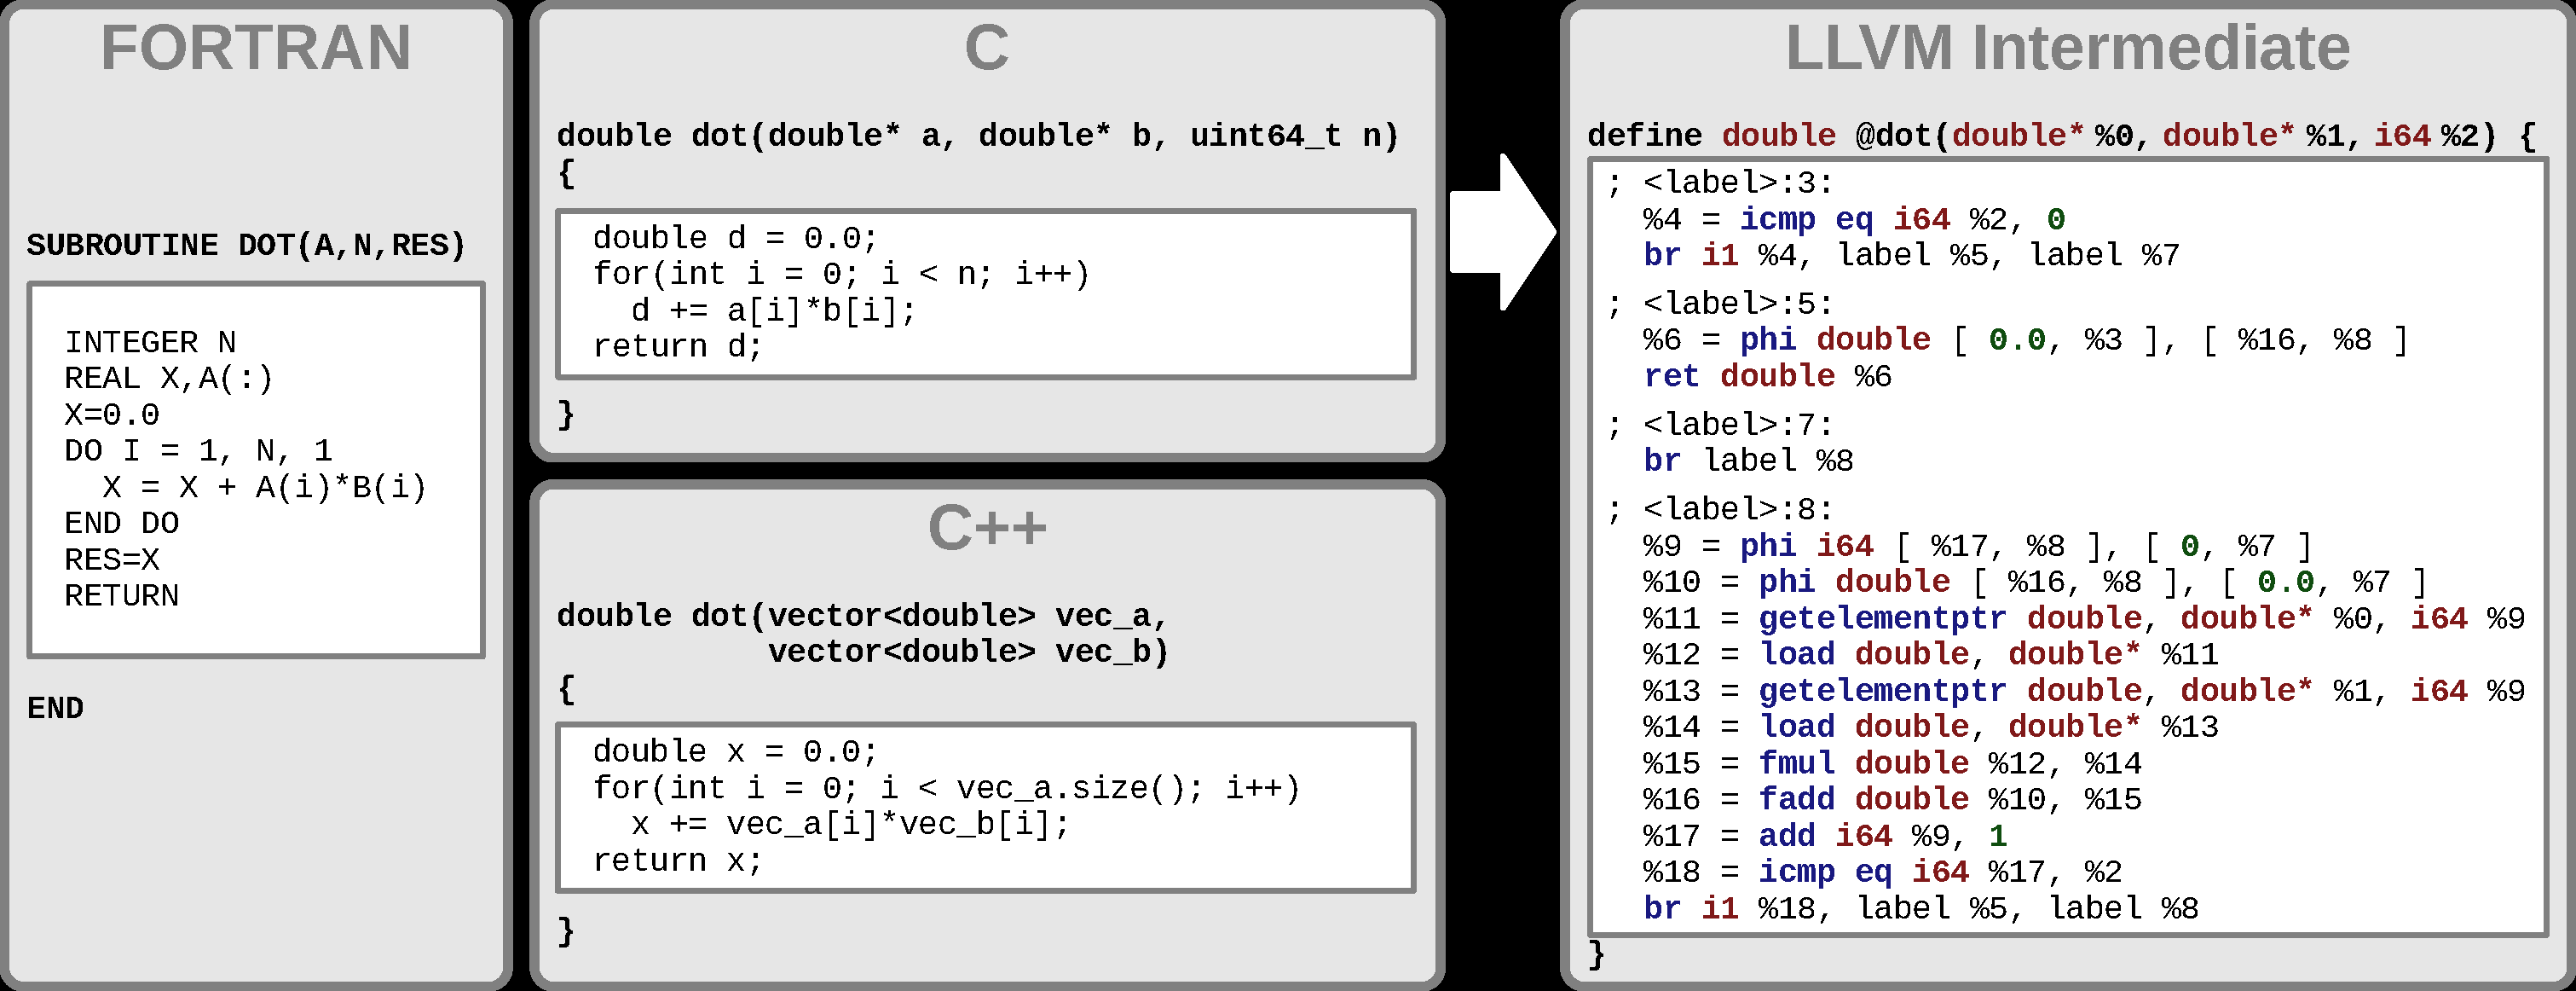
\includegraphics[width=\columnwidth]{figures/model_representations_textual}
\end{blackbox}

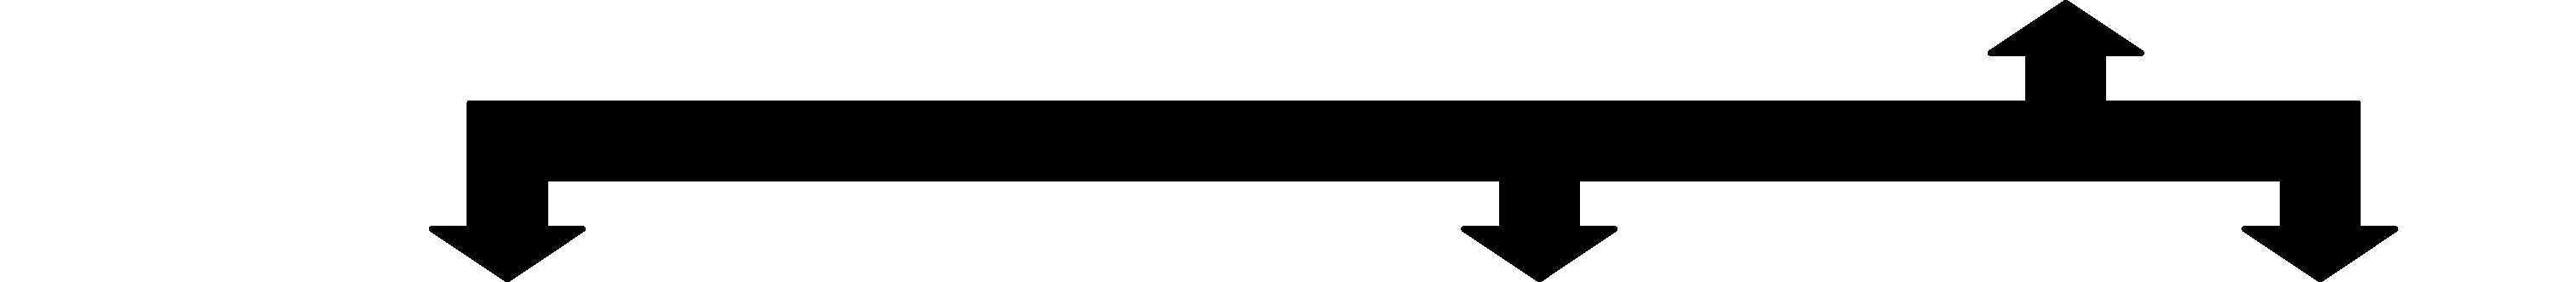
\includegraphics[width=\columnwidth]{figures/model_arrows_upper}

\begin{blackbox}{Data Structure Representation}
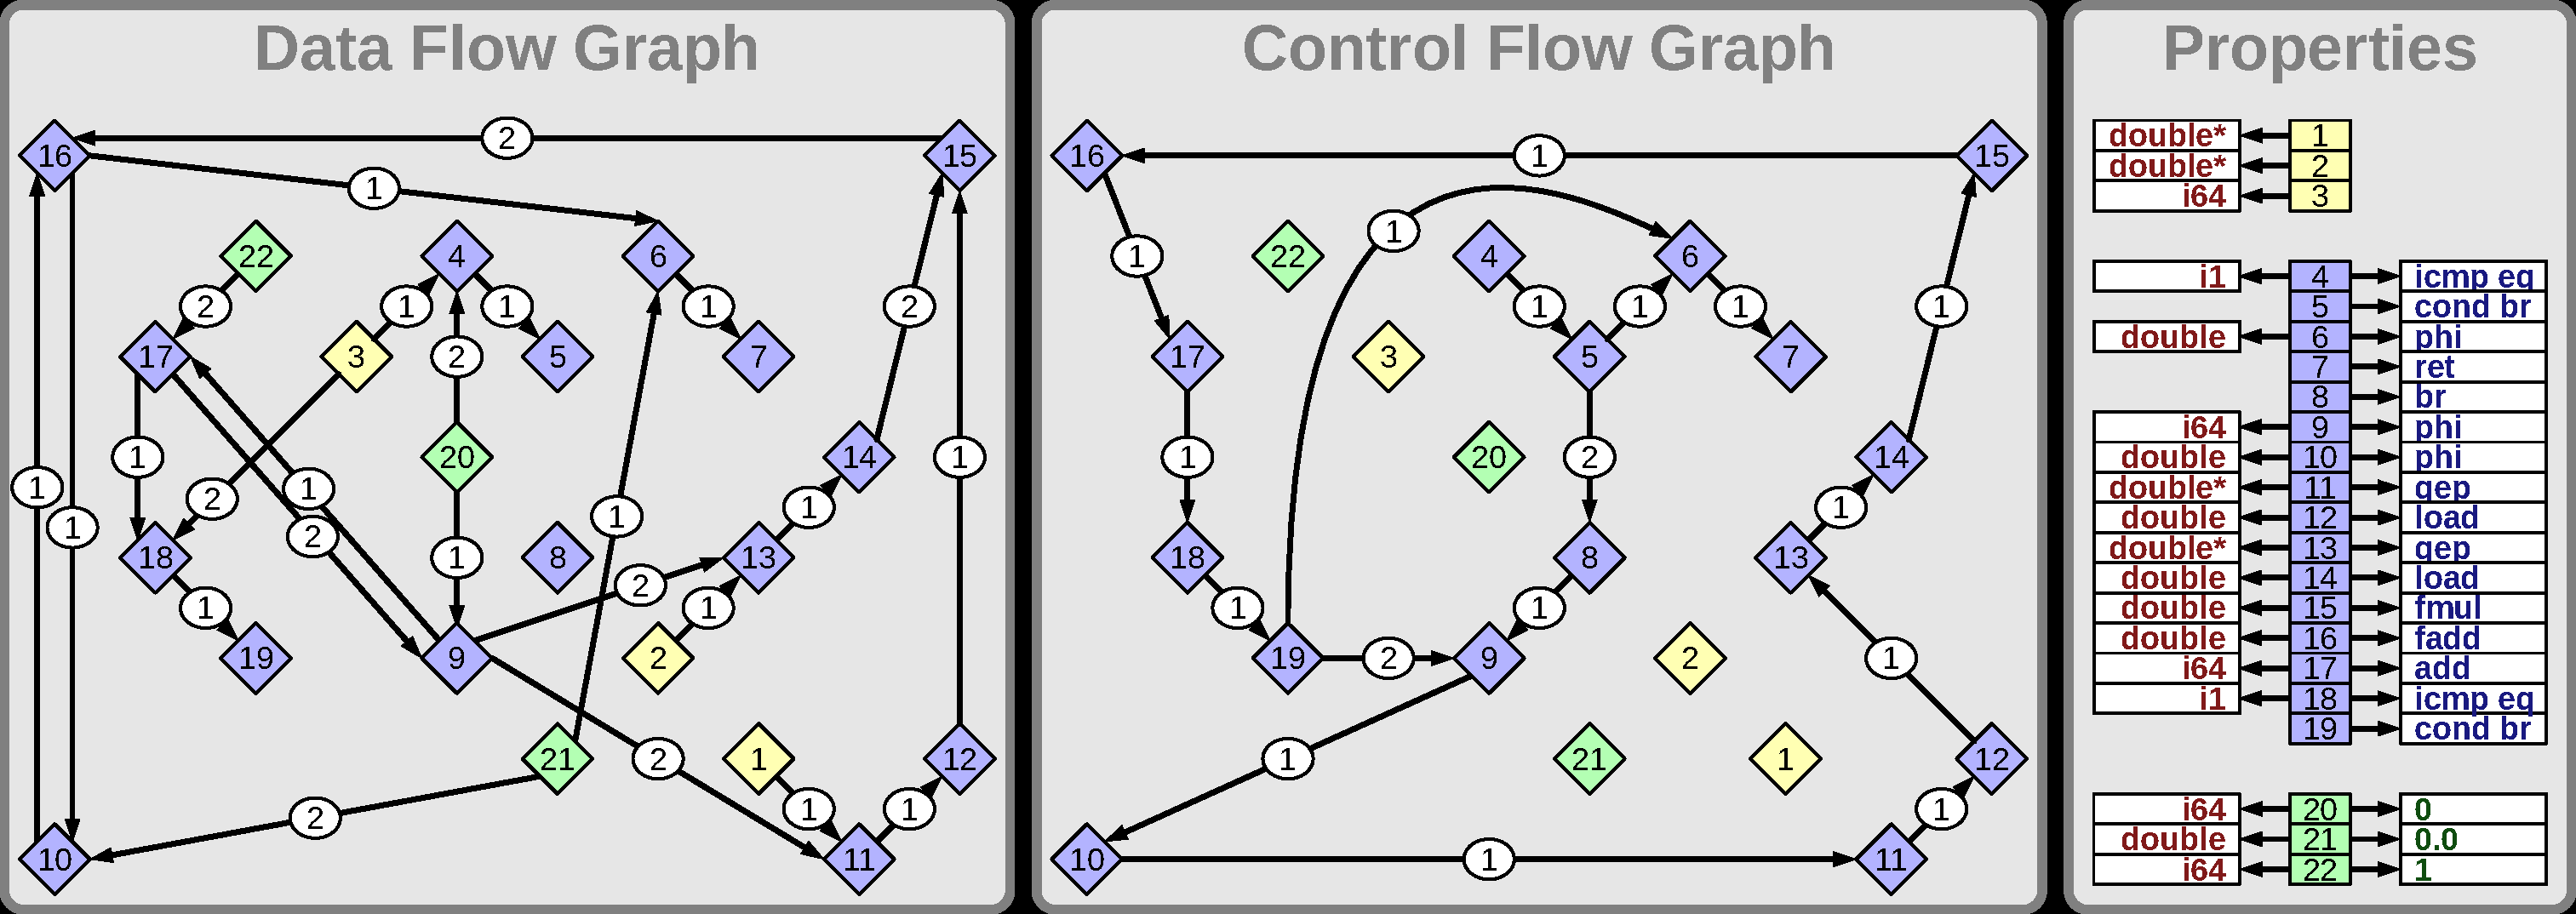
\includegraphics[width=\columnwidth]{figures/model_representations_structure}
\end{blackbox}

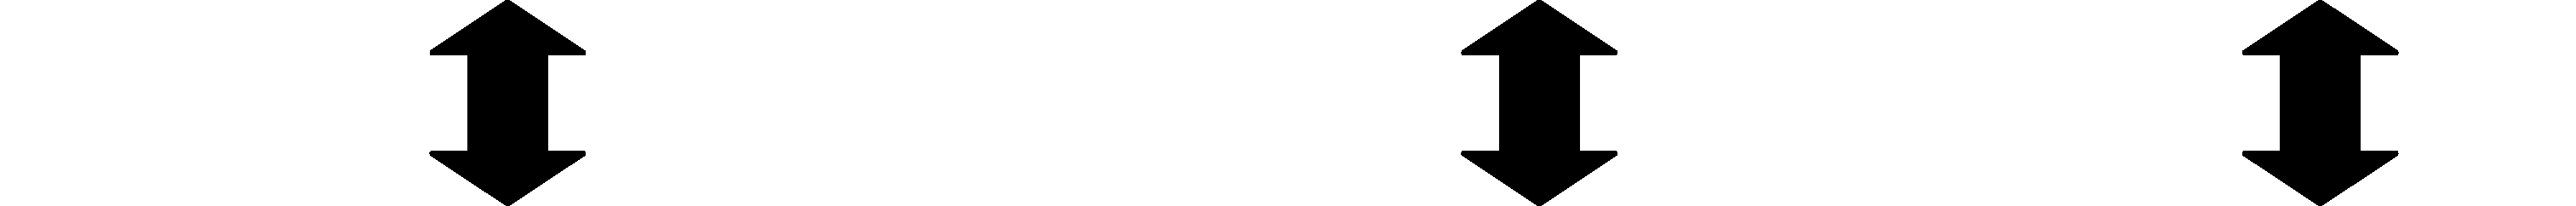
\includegraphics[width=\columnwidth]{figures/model_arrows_lower}

\begin{blackbox}{Mathematical Representation}
    \centering
    \begin{minipage}{0.329\textwidth}
        \begin{graybox}
            \scriptsize
            \setlength{\abovedisplayskip}{0pt}
            \setlength{\belowdisplayskip}{0pt}
            \vspace{-0.5em}
            \begin{align*}
                DF&G_\mathcal F=\{(1,11,1),(2,13,1)\\[-0.5em]
                  &(3,4,1),(3,18,2),(4,5,1),\\[-0.5em]
                  &(6,7,1),(9,11,2),(9,13,2),\\[-0.5em]
                  &(9,17,1),(10,16,1),(11,12,1),\\[-0.5em]
                  &(12,15,1),(13,14,1),(14,15,2),\\[-0.5em]
                  &(15,16,2),(16,6,1),(16,10,1),\\[-0.5em]
                  &(17,9,2),(17,18,1),(18,19,1),\\[-0.5em]
                  &(20,4,2),(20,9,1),(21,6,1),\\[-0.5em]
                  &(21,10,2),(22,17,2)\}\subset\mathbb N^3
            \end{align*}
        \end{graybox}
    \end{minipage}
    \begin{minipage}{0.329\textwidth}
        \begin{graybox}
            \scriptsize
            \setlength{\abovedisplayskip}{0pt}
            \setlength{\belowdisplayskip}{0pt}
            \vspace{-0.5em}
            \begin{align*}
                CFG_\mathcal F=\{&(4,5,1),(5,6,1),\\[-0.5em]
                  &(5,8,2),(6,7,1),\\[-0.5em]
                  &(8,9,1),(9,10,1),\\[-0.5em]
                  &(10,11,1),(11,12,1),\\[-0.5em]
                  &(12,13,1),(13,14,1),\\[-0.5em]
                  &(14,15,1),(15,16,1),\\[-0.5em]
                  &(16,17,1),(17,18,1),\\[-0.5em]
                  &(18,19,1),(19,6,1),\\[-0.5em]
                  &(19,9,2)\}\subset\mathbb N^3
            \end{align*}
        \end{graybox}
    \end{minipage}
    \begin{minipage}{0.329\textwidth}
        \centering
        \begin{graybox}
            \scriptsize
            \setlength{\abovedisplayskip}{0pt}
            \setlength{\belowdisplayskip}{0pt}
            \vspace{-0.5em}
            \begin{align*}
                T_\mathcal F={}&\{(1,\textit{double*}),(2,\textit{double*}),\dots\}\\[-0.5em]
                      \subset{}&\mathbb N\times Types_\text{LLVM}\\[-0.25em]
                P_\mathcal F={}&\{1,2,3\}\subset\mathbb N\\[-0.25em]
                I_\mathcal F={}&\{(4,\textit{icmp eq}),(5,\textit{cond br}),\dots\}\\[-0.5em]
                      \subset{}&\mathbb N\times Opcodes_\text{LLVM}\\[-0.25em]
                G_\mathcal F={}&\{\}\subset\mathbb N\\[-0.25em]
                C_\mathcal F={}&\{(20,0),(21,0),(22,1)\}\\[-0.5em]
                      \subset{}&\mathbb N\times\mathbb R
            \end{align*}

            \vspace{0.45em}
        \end{graybox}
    \end{minipage}

    \begin{minipage}{0.55\textwidth}
        \begin{graybox}
            \setlength{\abovedisplayskip}{0pt}
            \setlength{\belowdisplayskip}{0pt}
            \vspace{-0.5em}
            \begin{align*}
                M_{dot}=(DFG_\mathcal{F},
                 CFG_\mathcal{F},
                 T_\mathcal{F},
                 P_\mathcal{F},
                 I_\mathcal{F},
                 G_\mathcal{F},
                 C_\mathcal{F})
            \end{align*}
        \end{graybox}
    \end{minipage}
\end{blackbox}
\caption{Compiler-generated LLVM IR code is decomposed into data flow, control
         flow and per-value attributes.
         Mathematical notations of the three components are shown at the
         bottom.}
\label{fig:derivemaths}
\end{figure}

\section{Constraint Programming on SSA Programs}
\label{sec:constraintprogramming}

    Properties of SSA programs can now be formulated as constraint problems on
    the SSA model.
    For this purpose, the {\it set of SSA models} is introduced in
    \Cref{def:modelrepresentations}, which \Cref{def:cprob} then uses to
    formulate {\em SSA constraint problem}s.

\begin{figure}[H]
\begin{definition}{Set of SSA Models}{modelrepresentations}
    Given a specific SSA representation (LLVM, Hydrogen, MIR, $\dots$),
    denote $F$ the set of all valid functions that can be expressed in it.

    The {\em set of SSA models} $\mathcal M$ is defined as
    \begin{align*}
        \mathcal M=\{M\mid M \text{ is the SSA model of some }\mathcal F\in F\}
    \end{align*}
\end{definition}

\begin{definition}{SSA constraint problem}{cprob}
    An {\it SSA constraint problem} $(V,C)$ is a pair of a finite set of
    variables $V$ and a boolean predicate
    $C\colon\mathcal M\times\mathbb N^V\mapsto\{1,0\}$.
    The set of {\em constraint solutions} for a given constraint problem and a
    specific SSA model $M\in\mathcal M$ is given as
    \begin{align*}
        S_M(V,C) = \{s\in\mathbb N^V\mid C(M,s)=1\}.
    \end{align*}
\end{definition}
\end{figure}

    Some intuition is required here.
    The predicate function $C$ takes two arguments, firstly the model of a
    function and secondly a tuple of integers from $\mathbb N^V$.
    The tuple has one integer for each element in $V$ and each integer
    corresponds to a value in the function that $M$ models via indexing
    into the set of used values.
    The predicate function determines whether these values are in a specific
    relationship to each other in the SSA model.
    Finally, the set of constraint solutions lists all those tuples for which
    the predicate holds.

\subsection{Constraint Program Example}

\begin{figure}[p]
    
\raggedright
{\bf(a)} {} Initial problem statement:\\[1em]

\centering
{\LARGE$\underbrace{\text{Detect\vphantom{p}}}
                  _{\text{solver }S}
      \ \underbrace{\text{simple loop iterators}}
                  _{\text{SSA constraint problem }(V,C)}
                  \ \text{in the}
      \ \underbrace{\text{dot product function}}
                  _{\text{SSA model }M_{dot}}
                    \text{.}$}\\[2em]

\raggedright
{\bf(b)} {} Formulation as constraint problem:\\[1em]

\centering
\fontsize{60}{0}$S{}$\fontsize{20}{0}$\left(
\begin{minipage}{0.8\textwidth}
    \normalsize
    \begin{blackwhitebox}{\Large SSA constraint problem}
        \setlength{\abovedisplayskip}{0pt}
        \setlength{\belowdisplayskip}{0pt}
        \vspace{-0.5em}
        \begin{align*}
            V={}&\{\text{phi}, \text{update}, \text{step}\}\\
            C(M,x)={}&    ((1,x_\text{step})
                            \in C_\mathcal{F}\mathrel\land
                           (add,x_\text{update})
                            \in I_\mathcal{F}\mathrel\land\\
               &\phantom{(}(x_\text{phi},x_\text{update})
                            \in DFG_\mathcal{F}^*\mathrel\land
                           (x_\text{step},x_\text{update})
                            \in DFG_\mathcal{F}^*\mathrel\land\\
               &\phantom{(}(x_\text{update},x_\text{phi})
                            \in DFG_\mathcal{F}^*\mathrel\land
                           (phi,x_\text{phi})
                            \in I_\mathcal{F})
        \end{align*}
    \end{blackwhitebox}
    \begin{blackwhitebox}{\Large SSA model}
        \setlength{\abovedisplayskip}{0pt}
        \setlength{\belowdisplayskip}{0pt}
        \vspace{-0.5em}
        \begin{align*}
            DF&G_\mathcal F=\{(1,1,11),(1,2,13),(1,3,4),(2,3,18),(1,4,5),(1,6,7),\\[-0.5em]
              &(2,9,11),(2,9,13),\underline{(1,9,17)},(1,10,16),(1,11,12),(1,12,15),\\[-0.5em]
              &(1,13,14),(2,14,15),(2,15,16),(2,16,6),(2,16,10),\underline{(2,17,9)},\\[-0.5em]
              &(1,17,18),(1,18,19),(2,20,4),(1,20,9),(1,21,6),(1,21,10),\\[-0.5em]
              &\underline{(2,22,17)}\}\\[-0.25em]
            CF&G_\mathcal F=\{(1,4,5),(1,5,6),(2,5,8),(1,6,7),(1,8,9),(1,9,10),\\[-0.5em]
              &(1,10,11),(1,11,12),(1,12,13),(1,13,14),(1,14,15),\\[-0.5em]
              &(1,15,16),(1,16,17),(1,17,18),(1,18,19),(1,19,6),(2,19,9)\}\\[-0.25em]
            T_\mathcal F&{}=\{(\textit{double*},1),(\textit{double*},2),\dots\}\\[-0.25em]
            P_\mathcal F&{}=\{1,2,3\}\\[-0.25em]
            I_\mathcal F&{}=\{(\textit{icmp eq},4),(\textit{cond br},5),(\textit{phi},6),(\textit{ret},7),(\textit{br},8),\underline{(\textit{phi},9)},\\[-0.5em]
                        &(\textit{phi},10),(\textit{gep},11),(\textit{load},12),(\textit{gep},13),(\textit{load},14),(\textit{fmul},15),\\[-0.5em]
                        &(\textit{fadd},16),\underline{(\textit{add},17)},(\textit{icmp eq},18),(\textit{cond br},19)\}\\[-0.25em]
            G_\mathcal F&{}=\{\}\\[-0.25em]
            C_\mathcal F&{}=\{(0,20),(0,21),\underline{(1,22)}\}
        \end{align*}
    \end{blackwhitebox}
\end{minipage}
\right)$\\[2em]

\raggedright
\normalsize
{\bf(c)} {} Resulting set of constraint solutions:\\[1em]

\centering
{\LARGE$S_{M_{dot}}(V,C)=\{\{\text{phi}\mapsto9,
                             \text{update}\mapsto17,
                             \text{step}\mapsto22\}\}\subset\mathbb N^V$}
\caption{Detection of simple loop iterators is formulated as a constraint
         problem and applied to the SSA model from \Cref{fig:derivemaths}.
         One solution corresponding to the source variable {\tt i} is found.}
\label{fig:constraintsolution}
\end{figure}

    Consider the task of detecting in a program all simple loop iterators in a
    function, shown in \Cref{fig:constraintsolution}.
    The top {\bf a)} demonstrates how this can be translated into a constraint
    problem, solved in the context of an SSA model.
    For demonstration purposes, the SSA model that was derived in
    \Cref{fig:derivemaths} is used.

    Simple loop iterators show up in LLVM IR as data flow cycles with a phi node
    and an add instruction.
    This is expressed as a constraint problem at the top of the second part
    {\bf b)} of the figure.
    The formulation introduces the variables
    $V=\{\text{phi}, \text{update}, \text{step}\}$ and a predicate to
    describe the required conditions on the variables.
    The predicate is decomposed with logical conjunctions (``$\land$'') into
    several {\em element-of} relationships that have to hold simultaneously on
    the structures of the model.
    Explicit control flow constraints for establishing the loop strucure are not
    required, as the data flow with the $\Phi$ node already implies the presence
    of a loop structure.
    Below the predicate formulation is the SSA model from
    \Cref{fig:derivemaths}.

    At the bottom {\bf c)} of the figure, the set of constraint solutions is
    shown.
    It contains as its only element the tuple
    $\{\text{phi}\mapsto6,\text{update}\mapsto14,\text{step}\mapsto19\}$.
    Note that elements of $\mathbb N^V$ can be identified as mappings
    $V\rightarrow\mathbb N$.
    The underlined strucures in the lower part of
    \Cref{fig:constraintsolution} {\bf b)} demonstrate the validity of the
    solution:
    $(1,22)\in C_\mathcal F$ and $(1,9,17)\in DFG_\mathcal F$ and
    $(2,22,17)\in DFG_\mathcal F$ and $(\textit{phi},9)\in I_\mathcal F$ and
    $(\textit{add},17)\in I_\mathcal F$ and $(2,17,9)\in DFG_\mathcal F$,
    corresponding to the six simple constraints that make up the predicate.

    Each solution therefore assigns an integer to each variable.
    With the help of \Cref{fig:derivemaths}, the specific values $9,17,22$
    can be identified with lines 14 and 17, as well as the constant 1 in the
    LLVM IR code from \Cref{llvmirexample} {\bf b)}.
    This corresponds to the loop iterator \texttt{i} in the C source code of the
    \texttt{dot} function, correctly identifying the only simple loop iterator.

    With a detailed derivation of the SSA model completed and some intuition
    about the nature of constraint problems, only the solver $S$ in
    \Cref{fig:constraintsolution} remains a black box.
    The next sections derive how a backtracking solver can
    be used to efficiently compute the set of solutions.

\section{Solving of SSA Constraint Problems}
\label{sec:constraintsolving}

    A solver for SSA constraint problems needs to efficiently compute $S_M(V,C)$
    for some concrete $(V,C)$ and $M$.
    This is a search problem:
    All values in $\mathbb N^V$ that satisfy $C$ with the context $M$ need to
    be identified.

    $\mathbb N^V$ is infinitely large, although the relevant search space can
    immediately be trimmed to only tuples that have all values $\leq|vals|$.
    The case \mbox{$|V|>50$} is common in later section, and \mbox{$|vals|>100$}
    is likely for interesting SSA functions.
    The remaining search space therefore still has $100^{50}=10^{100}$ elements.
    This means that a brute force search is unfeasible, even assuming that
    the direct evaluation of $C$ for any potential solution can be performed
    efficiently for any candidate.
    However, backtracking can be used to find partial solutions, which are
    incrementally extended.
    This prunes the search space more effectively.

\begin{figure}[h]
    \begin{definition}{Backtracking Solution of Constraint Problems}{backtracking}
        Given a constraint problem $(V,C)$, an order $V=\{v_1,\dots,v_n\}$ with
        the corresponding projections $p_k\colon\mathbb N^V\rightarrow\mathbb N^k$,
        $x\mapsto(x_{v_1},\dots x_{v_k})$ can be choosen.
        Then a collection $(P_k)_{k=1\dots n}$ of functions
        $P_k:\mathcal M\times \mathbb N^{k-1}\times\rightarrow\mathcal P(\mathbb N)$,
        where $\mathcal P(\mathbb N)$ is the set of all subsets of $\mathbb N$,
        is a {\em backtracking solution} of $(V,C)$ if and only if for all
        $x\in\mathbb N^V$ the following is satisfied
        \begin{align}
            C(M,x)=1\iff\left[x_{v_k}\in P_k(M,p_{k-1}(x))=1\text{ for all }1\leq k\leq n\right].
        \end{align}
    \end{definition}
\end{figure}

    Note that \Cref{def:backtracking} defines the concept of a backtracking
    solution, but it does not show how such a backtracking solution could
    actually be constructed.
    That is a topic of later sections.
    In this context, the concept is introduced in order to allow the definition
    of the backtracking search \Cref{backtrackalg}, which operates as
    follows.
    The variable $x$ iterates over $\mathbb N^n$
    (which is identified with $\mathbb N^V$ in line 7), while the variable $k$
    tracks the number of currently considered dimensions of this partial
    solution.
    After initialisation in line 2, a single loop spans the remainder of the
    algorithm.
    In each iteration, the algorithm tries to assign a valid value to the latest
    element in the partial solution in line 4.
    By convention, the minimum of an empty set yields the symbol ``$\infty$''.
    If this occurs, the algorithm backtracks in lines 12--17.
    Otherwise, the solution is either complete (lines 6--8), or the algorithm
    increases the size of the partial solution in lines 9--11 and continues the
    search for the next element of $x$ in the following iteration.

\begin{algorithm}[p]
    \caption{Basic backtracking algorithm}
    \begin{algorithmic}[1]
        \Procedure{Detect}{$M,(P_k)_{k=1\dots n}$}\vspace{-0.45em}
            \State $k\gets1$,\quad$x\gets(1,\dots,1)\in\mathbb N^n$\vspace{-0.45em}
            \While{$true$}\vspace{-0.45em}
                \State $x_k\gets min\{y\in P_k(M,p_{k-1}(x))\mid y\geq x_k\}$\vspace{-0.45em}
                \If{$x_k<\infty$}\vspace{-0.45em}
                    \If{$k=n$}\vspace{-0.45em}
                        \State {\bf yield} $\{v_k\mapsto x_k\}_{k=1\dots n}\in\mathbb N^V$\vspace{-0.45em}
                        \State $x_k\gets x_k+1$\vspace{-0.45em}
                    \Else\vspace{-0.45em}
                        \State $k\gets k+1$\vspace{-0.45em}
                        \State $x_k\gets1$\vspace{-0.45em}
                    \EndIf
                \Else\vspace{-0.45em}
                    \State $k\gets k-1$\vspace{-0.45em}
                    \If{$k\geq1$}\vspace{-0.45em}
                        \State$x_k\gets x_k+1$\vspace{-0.45em}
                    \Else\vspace{-0.45em}
                        \State {\bf exit}
                    \EndIf
                \EndIf
            \EndWhile
        \EndProcedure
    \end{algorithmic}
    \label{backtrackalg}
\end{algorithm}

\subsection{Structure of Basic SSA Constraint Problems}

    Basic construction rules for SSA constraint problems are the
    element-of constraint problem in \Cref{def:elementofconstr}
    and the conjunction and disjunction constraint problems in
    \Cref{def:conjconstr}.
    \Cref{def:constrext} enables conjunctions or disjunctions of constraint
    problems that are not defined the same set of variables.
    The example in \Cref{fig:constraintsolution} can be constructed with only
    these rules.

\begin{figure}[p]
    \begin{definition}{Element-of Constraint Problem}{elementofconstr}
        For a set of tuples $S(M)\subset\mathbb N^V$ that is potentially
        dependent on the SSA model $M\in\mathcal M$
        (i.e.\ $S(M):=DFG_\mathcal F^*$),
        the element-of constraint problem $(V,E_S)$ is given by
        \begin{align*}
            E_S(M,x)=\left\{\begin{array}{l}
                                1\text{\quad if }x \in S(M)\\
                                0\text{\quad otherwise}.
                            \end{array}\right.
        \end{align*}
    \end{definition}

    \begin{definition}{Conjunction and Disjunction Constraint}{conjconstr}
        For two constraint problems $(V,C)$ and $(V,C')$, the
        conjunction constraint $(V,C\mathrel\land C')$ and the
        disjunction constraint $(V,C\mathrel\lor C')$ are given by
        \begin{align*}
            &C\mathrel\land C'(M,x)=\left\{
                \begin{array}{l}
                    1\text{\quad if }C(M,x)=1\mathrel\land C'(M,x)=1\\
                    0\text{\quad otherwise}
                \end{array}\right.\\
            &C\mathrel\lor C'(M,x)=\left\{
                \begin{array}{l}
                    1\text{\quad if }C(M,x)=1\mathrel\lor C'(M,x)=1\\
                    0\text{\quad otherwise}.
                \end{array}\right.
        \end{align*}
    \end{definition}

    \begin{definition}{Extension of Constraint Problems}{constrext}
        For an SSA constraint problem $(V,C)$ and an injection
        $i:V\hookrightarrow W$, the constraint problem $(W,C^W)$ is given by
        \begin{align*}
            C^W(M,x)=C(M,\{x_{i(v)}\}_{v\in V}).
        \end{align*}
    \end{definition}
\end{figure}

\begin{figure}[p]
    \begin{theorem}{Backtracking Solution for Element-of Constraint Problems}{theo1}
    For $S\subset\mathbb N^V$, the functions $(P_k[E_S])_{k=1\dots n}$,
    $P_k[E_S]\colon\mathcal M\times\mathbb N^{k-1}\rightarrow\mathcal P(\mathbb N)$
    defined by
    \begin{align*}
        P_k[E_S](M,x)=head(R_k(M,x))
    \end{align*}
    give a backtracking solution of $(V,E_S)$, where
    $R_k(M,x)\subset\mathbb N^{n-k+1}$ is given by
    \begin{align*}
        R_k(M)={}&\{p_n(s)\mid s\in S(M)\}\\
        R_{k+1}(M,x)={}&select(x_k,R_k(M,(x_1,\dots,x_{k-1}))).
    \end{align*}
    \tcblower
    \paragraph*{Proof:} By definition,
    $E_S(M,x)=1\iff x\in S(M)\iff p_n(x)\in\{p_n(s)\mid s\in S(M)\}$.
    It is also clear that for all $1\leq k\leq n$ holds
    \begin{align*}
        p_n(x)\in\{p_n(s)\mid s\in S(M)\}\iff p_n(x)\in\{p_n(s)\mid s\in S(M),p_{k-1}(s)=p_{k-1}(x)\}.
    \end{align*}
    For all $1\leq k\leq n$, this together gives
    \begin{align*}
        E_S(M,x)=1\implies x_{v_k}\in\{s_{v_k}\mid s\in S(M),p_{k-1}(s)=p_{k-1}(x)\}=P_k[E_S](M,p_{k-1}(x)).
    \end{align*}

    This gives ``$\implies$'' for the equation in \Cref{def:backtracking}.
    The reverse is true for $k=n$, as
    \begin{align*}
        x_{v_n}\in{}&\{s_{v_n}\mid s\in S(M),p_{k-1}(s)=p_{k-1}(x)\}\implies x\in S(M).
    \end{align*}
    Therefore, the equivalence from \Cref{def:backtracking} holds in both directions.
\end{theorem}
\begin{theorem}{Backtracking Solution for Conjunction Constraint problems}{theo2}
    For SSA constraint problems $(V,C)$ and $(V,C')$ with backtracking
    solutions $(P_k)_{k=1\dots n}$, $(P'_k)_{k=1\dots n}$, the
    functions $(P_k[C\mathrel\land C'])_{k=1\dots n}$,
    $P_k[C\mathrel\land C']\colon\mathcal M\times\mathbb N^{k-1}\rightarrow\mathcal P(\mathbb N)$
    defined by
    \begin{align*}
        P_k[C\mathrel\land C'](M,x)=P_k(M,x)\mathrel\cap P'_k(M,x)
    \end{align*}
    give a backtracking solution of $(V,C\mathrel\land C')$.
    \tcblower
    \paragraph*{Proof:}
    The definition of $(V,C\mathrel\land C')$ together with the
    assumption that \Cref{def:backtracking} holds for the two given
    backtracking solutions gives
    \begin{align*}
        C\mathrel\land C'(M,x)=1\iff{}&\left[x_{v_k}\in P_k(M,p_{k-1}(x))\text{ for all }1\leq k\leq n\right]\\
                              \mathrel\land{}&\left[x_{v_k}\in P'_k(M,p_{k-1}(x))\text{ for all }1\leq k\leq n\right].
    \end{align*}
    With the definition of $P_k[C\mathrel\land C']$, this immediately gives
    \begin{align*}
        C\mathrel\land C'(M,x)=1\iff\left[x_{v_k}\in P_k[C\mathrel\land C'](M,(x_{v_1},\dots,x_{v_{k-1}}),x_{v_k})\text{ for all }1\leq k\leq n\right].
    \end{align*}
\end{theorem}

\end{figure}

\begin{figure}[p]
    \begin{theorem}{Backtracking Solution for Disjunction Constraint problems}{theo3}
    For SSA constraint problems $(V,C)$ and $(V,C')$ with backtracking
    solutions $(B_k)_{k=1\dots n}$, $(B'_k)_{k=1\dots n}$, the collection
    $(B_k[C\hspace{-0.5mm}\lor\hspace{-0.5mm}C'])_{k=1\dots n}$ of functions
    \mbox{$B_k[C\hspace{-0.5mm}\lor\hspace{-0.5mm}C']\colon\mathcal M\times\mathbb N^{k-1}\rightarrow\mathcal P(\mathbb N)$}
    is a backtracking solution of
    $(V,C\hspace{-0.5mm}\lor\hspace{-0.5mm}C')$ when defined by
    \begin{align*}
        B_k[C\hspace{-0.5mm}\lor\hspace{-0.5mm}C'](M,x)=\left(\left\{
            \begin{array}{ll}
                B_k(M,x)&\text{if }R_{k,1}(M,x)\\
                \emptyset&\text{otherwise}
            \end{array}\right.
            \right)\cup\left(\left\{
            \begin{array}{ll}
                B'_k(M,x)&\text{if }R_{k,2}(M,x)\\
                \emptyset&\text{otherwise}
            \end{array}\right.
            \right)
    \end{align*}
    \vspace{-0.2cm}
    \begin{align*}
        R_1(M)=\left(\begin{array}{l}1\\1\end{array}\right)&&
        R_{k+1}(M,x,x_k)=\left(
            \begin{array}{l}
                R_{k,1}(M,x)\mathrel\land x_k\in B_k(M,x)\\
                R_{k,2}(M,x)\mathrel\land x_k\in B'_k(M,x)
            \end{array}\right).
    \end{align*}
    \tcblower
    \paragraph*{Proof:}
    The equivalence from \Cref{def:backtracking} holds for the backtracking
    solutions of $(V,C)$, $(V,C')$ by assumption.
    With $C\hspace{-0.5mm}\lor\hspace{-0.5mm}C'(M,x)=1\iff C(M,x)=1\mathrel\lor C'(M,x)=1$,
    this gives
    \begin{align*}
        C\hspace{-0.5mm}\lor\hspace{-0.5mm}C'(M,x)=1\iff{}&x_{v_k}\in B_k(M,p_{k-1}(x))\text{ for all }1\leq k\leq n\\
                                            \mathrel\lor{}&x_{v_k}\in B'_k(M,p_{k-1}(x))\text{ for all }1\leq k\leq n.
    \end{align*}
    After expanding $R_k$, this directly corresponds to the definition of
    $B_n[C\hspace{-0.5mm}\lor\hspace{-0.5mm}C']$.
    Therefore
    \begin{align*}
        C\hspace{-0.5mm}\lor\hspace{-0.5mm}C'(M,x)=1\iff{}x_{v_n}\in B_n[C\hspace{-0.5mm}\lor\hspace{-0.5mm}C'](M,p_{n-1}(x)).
    \end{align*}
    This is sufficient for the equivalence in \Cref{def:backtracking} to hold
    in both directions, as for all $1\leq k\leq n$, the definition of
    $B_k[C\hspace{-0.5mm}\lor\hspace{-0.5mm}C']$ with expanded $R_k$ directly
    gives
    \begin{align*}
        x_{v_n}\in B_n[C\hspace{-0.5mm}\lor\hspace{-0.5mm}C'](M,p_{n-1}(x))\implies x_{v_k}\in B_k[C\hspace{-0.5mm}\lor\hspace{-0.5mm}C'](M,p_{k-1}(x)).
    \end{align*}
\end{theorem}
\begin{theorem}{Backtracking Solution for Extensions of Constraint Problems}{theo4}
    For an SSA constraint problem $(V,C)$ with a backtracking
    solution $(B_k)_{k=1\dots n}$ and a set $W$ with an injection
    $i:V\hookrightarrow W$ and an enumeration of $W=\{w_1,\dots,w_{|W|}\}$ that
    is compatible with the enumeration of $V$ such that $i(v_k)=w_{t(k)}$ with
    some $t:\mathbb N\rightarrow\mathbb N$ strictly increasing, the collection
    $(B_k[C^W])_{k=1\dots |W|}$ of functions
    $B_k[C^W]\colon\mathcal M\times\mathbb N^{k-1}\rightarrow\mathcal P(\mathbb N)$
    is a backtracking solution of $(V,C^W)$ when defined by
    \begin{align*}
        B_k[C^W](M,x)=\left\{
            \begin{array}{ll}
                B_k\left(M,\left(x_{t(1)},\dots,x_{t(k'-1)}\right)\right)&\text{if }k=t(k')\text{ for some }1\leq k'\leq|V|\\
                \mathbb N&\text{otherwise}\\
            \end{array}\right..
    \end{align*}
    \tcblower
    \paragraph*{Proof:}
    This follows immediately from \Cref{def:backtracking} and \Cref{def:constrext}.
\end{theorem}

\end{figure}

    \Cref{theo:theo1} introduces backtracking solutions for element-of
    constraint problems.
    They are constructed such that
    $P_k[E_S](M,x)=\{y_{v_k}\mid y\in S(M), y_{v_1}=x_1,\dots,y_{v_{k-1}}=x_{k-1}\}$.
    This is the optimal backtracking solution in the sense that the backtracking
    algorithm will only ever backtrack immediately after yielding a result.
    In the theorem, the backtracking solution is not defined directly, but
    instead a helper construct $R_k$ is introduced.
    This helper construct is used in \Cref{subsec:impl} for an efficient
    implementation.

    \Cref{theo:theo2} introduces backtracking solutions for conjunction
    constraint problems.
    These are defined in the obvious way, by taking the intersection of
    the underlying backtracking solitions at each $k$.
    This is not possible for disjunction constraint problems, which are dicussed
    in \Cref{theo:theo3}.
    The additional structure $R_k$ is used to keep track whether the current
    partial solution satisfies $C$ or $C'$ so far.
    The partial solution at $k$ is then the union only of those underlying
    partial solutions at $k$ where the corresponding element in $R_k$
    signals validity.

    \Cref{theo:theo3} shows that backtracking solutions for extensions of
    constraint problems can be constructed by simply ignoring the additional
    variables.

\subsection{Backtracking Example}

\begin{figure}[p]
    \centering
\begin{blackwhitebox}{Original SSA Constraint Problem}
    \setlength{\abovedisplayskip}{0pt}
    \setlength{\belowdisplayskip}{0pt}
    \vspace{-0.5em}
\begin{align*}
        V={}&\{\text{phi}, \text{update}, \text{step}\}\\
        C(M,x)={}&    ((1,x_\text{step})
                        \in C_\mathcal{F}\mathrel\land
                       (add,x_\text{update})
                        \in I_\mathcal{F}\mathrel\land\\
           &\phantom{(}(x_\text{phi},x_\text{update})
                        \in DFG_\mathcal{F}^*\mathrel\land
                       (x_\text{step},x_\text{update})
                        \in DFG_\mathcal{F}^*\mathrel\land\\
           &\phantom{(}(x_\text{update},x_\text{phi})
                        \in DFG_\mathcal{F}^*\mathrel\land
                       (phi,x_\text{phi})
                        \in I_\mathcal{F}
    \end{align*}
\end{blackwhitebox}

\vspace{1cm}
\begin{minipage}[t]{6cm}
    \centering
    {\Large\bf Backtracking Solution:}

    $k=1$\quad$v_1=\text{phi}$
    \begin{graybox}
        \setlength{\abovedisplayskip}{0pt}
        \setlength{\belowdisplayskip}{0pt}
        \vspace{-0.5em}
        \begin{align*}
            B_1[C](M)={}&heads(DFG_\mathcal{F}^*)\\
                \mathrel\cap{}&heads(rev(DFG_\mathcal{F}^*))\\
                \mathrel\cap{}&heads(select(phi,I_\mathcal{F}))
        \end{align*}
    \end{graybox}
    \vspace{-0.75em}
    \phantom{\Huge \rotatebox[origin=c]{330}{$\downarrow$}{}}
    \hspace{0.3cm}
    \phantom{\Huge\rotatebox[origin=c]{0}{$\downarrow$}}
    \hspace{0.3cm}
    \phantom{\Huge\rotatebox[origin=c]{30}{$\downarrow$}}

    $k=2$\quad$v_2=\text{update}$
    \begin{graybox}
        \setlength{\abovedisplayskip}{0pt}
        \setlength{\belowdisplayskip}{0pt}
        \vspace{-0.5em}
        \begin{align*}
            B_2[C]&(M,x)=\\
                            {}&heads(select(add,I_\mathcal{F}))\\
                \mathrel\cap{}&heads(select(x_1,DFG_\mathcal{F}^*))\\
                \mathrel\cap{}&heads(rev(DFG_\mathcal{F}^*))\\
                \mathrel\cap{}&heads(select(x_1,rev(DFG_\mathcal{F}^*)))
        \end{align*}
    \end{graybox}
    \vspace{-0.75em}
    \phantom{\Huge \rotatebox[origin=c]{330}{$\downarrow$}{}}
    \hspace{0.3cm}
    \phantom{\Huge\rotatebox[origin=c]{0}{$\downarrow$}}
    \hspace{0.3cm}
    \phantom{\Huge\rotatebox[origin=c]{30}{$\downarrow$}}

    $k=3$\quad$v_3=\text{step}$
    \begin{graybox}
        \setlength{\abovedisplayskip}{0pt}
        \setlength{\belowdisplayskip}{0pt}
        \vspace{-0.5em}
        \begin{align*}
            B_3[C]&(M,x)=select(1,C_\mathcal{F})\\
                \mathrel\cap{}&heads(select(x_2,rev(DFG_\mathcal{F}^*)))
        \end{align*}
    \end{graybox}
    \vspace{-0.75em}
    \phantom{\Huge \rotatebox[origin=c]{330}{$\downarrow$}{}}
    \phantom{\Huge\rotatebox[origin=c]{0}{$\downarrow$}}
    \phantom{\Huge\rotatebox[origin=c]{30}{$\downarrow$}}

    \phantom{\large $x=(9,17,22)$}
\end{minipage}
\hfill
\begin{minipage}[t]{8cm}
    \centering
    {\Large\bf Backtracking Algorithm:}

    \begin{minipage}{4cm}
        \centering
        \vspace{1.9mm}
        $x=()$
        \begin{graybox}
            \setlength{\abovedisplayskip}{0pt}
            \setlength{\belowdisplayskip}{0pt}
            \vspace{-0.5em}
            \begin{gather*}
                \\B_1[C](M)=\{6,9,10\}\\
            \end{gather*}
        \end{graybox}
        \vspace{-0.75em}
        {\Huge \rotatebox[origin=c]{330}{$\downarrow$}{}}
        \hspace{0.8cm}
        {\Huge\rotatebox[origin=c]{0}{$\downarrow$}}
        \hspace{0.8cm}
        {\Huge\rotatebox[origin=c]{30}{$\downarrow$}}
    \end{minipage}

    \begin{minipage}{2.5cm}
        \centering
        \vspace{0.7mm}
        $x=(6)$
        \begin{graybox}
            \setlength{\abovedisplayskip}{0pt}
            \setlength{\belowdisplayskip}{0pt}
            \vspace{-0.5em}
            \begin{gather*}
                \\B_2[C](M,6)\\=\\\{\}\\
            \end{gather*}
        \end{graybox}
        {\large\bf backtrack!}
    \end{minipage}
    \begin{minipage}{2.5cm}
        \centering
        \vspace{0.7mm}
        $x=(9)$
        \begin{graybox}
            \setlength{\abovedisplayskip}{0pt}
            \setlength{\belowdisplayskip}{0pt}
            \vspace{-0.5em}
            \begin{gather*}
                \\B_2[C](M,9)\\=\\\{17\}\\
            \end{gather*}
        \end{graybox}
        \vspace{-0.75em}
        \phantom{\Huge \rotatebox[origin=c]{330}{$\downarrow$}{}}
        {\Huge\rotatebox[origin=c]{0}{$\downarrow$}}
        \phantom{\Huge\rotatebox[origin=c]{30}{$\downarrow$}}
    \end{minipage}
    \begin{minipage}{2.5cm}
        \centering
        \vspace{0.7mm}
        $x=(10)$
        \begin{graybox}
            \setlength{\abovedisplayskip}{0pt}
            \setlength{\belowdisplayskip}{0pt}
            \vspace{-0.5em}
            \begin{gather*}
                \\B_2[C](M,10)\\=\\\{\}\\
            \end{gather*}
        \end{graybox}
        {\large\bf backtrack!}
    \end{minipage}

    \begin{minipage}{4cm}
        \centering
        \vspace{0.7mm}
        $x=(9,17)$
        \begin{graybox}
            \setlength{\abovedisplayskip}{0pt}
            \setlength{\belowdisplayskip}{0pt}
            \vspace{-0.5em}
            \begin{gather*}
                \\[-3.75mm]
                B_3[C](M,9,17)=\{22\}
                \\[-3.75mm]
            \end{gather*}
        \end{graybox}
        \vspace{-0.75em}
        \phantom{\Huge \rotatebox[origin=c]{330}{$\downarrow$}{}}
        {\Huge\rotatebox[origin=c]{0}{$\downarrow$}}
        \phantom{\Huge\rotatebox[origin=c]{30}{$\downarrow$}}
    \end{minipage}

    \vspace{0.5mm}
    {\large $x=(9,17,22)$}
\end{minipage}
    \caption{Backtracking is used to find the single solution of the SSA
             constraint problem from \Cref{fig:constraintsolution}.
             The partial solution is extended in three steps from top to bottom.
             The backtracking solution $(P_k[C])_{k=1\dots3}$ is contructed
             according to \Cref{theo:theo1,theo:theo2,theo:theo4}.}
    \label{fig:backtracsol}
\end{figure}

    \Cref{fig:backtracsol} shows how backtracking is used to algorithmically
    determine the solution of the SSA constraint problem that was introduced in
    \Cref{fig:constraintsolution}.
    The original SSA constraint problem is shown again at the top of the figure.
    It is entirely constructed via conjunctions of element-of constraint
    problems.
    The constraint problem can therefore be expressed entirely according to
    \Cref{def:elementofconstr,def:conjconstr,def:constrext}.

    This means that \Cref{theo:theo1,theo:theo2,theo:theo4} can be used to
    construct a backtracking solution $(P_k[C])_{k=1\dots3}$ of the constraint
    problem.
    The lower part of the figure demonstrates how this backtracking solution is
    used to determine the solution.

    Starting from the top with an empty partial solution, candidates for $x_1$
    are determined, corresponding to the variable {\em phi}.
    The SSA model contains three phi nodes, all of which also satisfy the other
    conditions of being the source and target of some edge in the data flow
    graph.
    Therefore, the algorithm continues with the partial solutions $x=(6)$,
    $x=(9)$ and $x=(10)$ one level further down in the figure.

    For $k=2$, which corresponds to the variable {\em update}, the backtracking
    solution requires $x_2$ to form a data flow loop with $x_1$.
    Futhermore, it requires it to be an $add$ instruction.
    The partial solution $(6)$ corresponds to a phi node that is not part of
    any data flow loop, therefore the algorithm backtracks.
    For the partial solution $(10)$, the phi node is part of a data flow loop
    only with the value $16$, but that value is an $fadd$ instruction.
    The partial solution $(9)$, however, can be extended according to the
    backtracking solution with the value $17$.
    Therefore, the algorithm continues at the bottom of the figure with only
    this single partial solution $(9,17)$.

    In order to complete this partial solution, $P_3[C]$ requires the value for
    the $step$ variable to be a constant of value $1$.
    Furthermore, is needs to be used as an argument to $x_2$, i.e.\ the
    $update$ variable.
    Both of these conditions hold for the value $22$, yielding a complete
    solution at the bottom of the figure.

\subsection{Implementation, Data Structures and Complexity}
\label{subsec:impl}

    With the concrete backtracking solutions that were derived in
    \Cref{theo:theo1,theo:theo2,theo:theo3,theo:theo4}, it is possible to
    identify suitable data structures and algorithmic decisions for efficiently
    implementing the corresponding functionality in real code.
    This first requires a revisiting of the backtracking algorithm first
    introduced in \Cref{backtrackalg}.
    \Cref{cppsolver} shows how this backtracking solver can be implemented as
    a C++ function.
    Most of the \texttt{solver} function in lines 12--43 maps directly onto
    \Cref{backtrackalg}, and needs no further explanation.
    However, there are some crucial details that are made explicit here, which
    need elaboration.
    They mostly relate to the calculation of
    $min\{y\in\mathbb N\mid y\geq x_k\mathrel\land P_k(\{x_1,\dots,x_{k-1},y\},M)=1\}$
    in line 4 of \Cref{backtrackalg}, which was previously left as a black
    box.

    \texttt{BacktrackingPart} corresponds to the backtracking solution in
    \Cref{def:backtracking}.
    The class provides four member functions.
    Most importantly, \texttt{skip\_invalid} is used for implementing the
    evaluation of
    $min\{y\in\mathbb N\mid y\geq x_k\mathrel\land P_k(\{x_1,\dots,x_{k-1},y\},M)=1\}$
    in line 4 of \Cref{backtrackalg}.
    More precisely, it increases the argument to the smallest value that is
    part of a partial solution.

\begin{figure}[p]
    \begin{lstlisting}[language=C++,,basicstyle=\linespread{0.9784}\ttfamily]
// This class corresponds to Definition 2.7.
class BacktrackingPart {
public:
  virtual SkipResult skip_invalid(unsigned& c) const;
  virtual void begin();
  virtual void fixate(unsigned c);
  virtual void resume();
};

void yield(const vector<int>& solution);
// The solver function corresponds to Algorithm 1.
void solver(vector<BacktrackingPart*> P) {
    int         k = 0;
    vector<int> x(P.size(), 0);
    while(true) {
        SkipResult result = P[k]->skip_invalid(x[k]);

        if(result == SkipResult::AMBIGUOUS)
            contintue;
        if(result != SkipResult::FAIL) {
            if(k + 1 == P.size())
            {
                yield(x);
                P[k]->resume();
                x[k]++;
            }
            else {
                P[k]->fixate(x[k]);
                k++;
                P[k]->begin();
                x[k] = 0;
            }
        }
        else {
            if(k > 0) {
                k = k - 1;
                P[k]->resume();
                x[k] = x[k] + 1;
            }
            else return {};
        }
    }
}
\end{lstlisting}

    \caption{Complete C++ implementation of \Cref{backtrackalg}.
             The if-else statements in lines 20--41 precisely correspond
             to those in lines 5--17 of that algorithm.
             The \texttt{BacktrackingPart} class provides
             $min\{y\in\mathbb N\mid y\geq x_k\mathrel\land P_k(\{x_1,\dots,x_{k-1},y\},M)=1\}$
             via \texttt{skip\_invalid}.
             The remaining member functions precompute structures that
             are used in \texttt{skip\_invalid} for quick evaluation.}
    \label{cppsolver}
\end{figure}

    The three other member function of \texttt{BacktrackingPart} manipulate
    state that is shared by the individual \texttt{BacktrackingPart} objects.
    This allows computations that would otherwise be performed repeatedly by
    the \texttt{skip\_invalid} function to instead of performed ahead of time.
    More specifically, this corresponds directly to $R_k(M,x)$ in both
    \Cref{theo:theo1} and \Cref{theo:theo4}.
    Crucially, this distribution of the computation allows all previously
    discussed types of SSA constraint problems to be implemented efficiently as
    follows.
    \begin{itemize}
    \item For element-of constraint problems, $R_k$ can be implemented as a
          tree structure, built around a sorted array of pairs.
          Each subtree in the array corresponds to a potential $R_{k+1}$.
          \begin{lstlisting}[language=C++]
struct Tree { vector<pair<int,Tree>> s; };
          \end{lstlisting}
          The \texttt{BacktrackingPart} implementation keeps an index into
          the array, which \texttt{begin} initialises.
          Each time \texttt{skip\_invalid} is called, the index is incremented
          until it either points to an entry $\geq$ the lower bound \texttt{c}
          or hits the end of the array.
          Finally, \texttt{resume} does nothing, and \texttt{fixate} simply
          accesses the array at the current index for the subtree $R_{k+1}$.
    \item For conjunction constraint problems, \texttt{begin}, \texttt{fixate}
          and \texttt{resume} call the corresponding members of the underlying
          \texttt{BacktrackingPart} objects, and \texttt{skip\_invalid}
          alternates between them until a fixpoint is reached or
          either of them fail.
    \item For disjunction constraints, $R_k$ is a pair of booleans.
          Calls to \texttt{skip\_invalid} are passed on to those underlying
          \texttt{BacktrackingPart} objects that are not disabled via $R_k$.
          If any succeeded, then the smallest resulting value is chosen.
          $R_k$ is updated in \texttt{fixate}, using the \texttt{skip\_invalid}
          results from before.
          The \texttt{begin}, \texttt{fixate} and \texttt{resume} member
          calls are also passed on to underlying objects
          that are enabled in $R_k$.
    \end{itemize}

    While the chosen data structures allow for very efficient implementations
    of the individual functions that are used to search for solutions, no
    meaningful limits can be put on computational complexity in general.
    This is due to the following observation:
    SSA constraint problems are a generalisation of the subgraph isomorphism
    problem, which is known to be NP-hard.

    However, this is not an impediment due to the nature of the use case.
    In practice, the nature of SSA constraint problems mean that a solver is
    going to solve the same limited set formulas repeatedly -- only in the
    context of different SSA models.
    This means that is it viable to craft the formulas in such a way to be
    efficiently solvable, in particular by choosing a good order in which to
    iterate over the variables.
    For specific SSA constraint problems, it can then be possible to give
    complexity assumptions.

\subsection{Additional SSA Constraint Problems}

    There are a number of additional construction rules for SSA constraint
    problems that are used in this thesis.
    Some of them are less intuitive than the previously introduced definitions,
    but allow for powerful compiler analysis.

    Firstly, there are a number of very simple SSA constraint problems that
    operate directly on the integer values, without interpreting them as indizes
    into the value list of the SSA model.
    These are listed in \Cref{def:auxconstr}.
    $(\{a,b\}, C^=)$ and $(\{a,b\}, C^{\neq})$ are defined in the
    obvious way, forcing equality/inequality.
    Finally, there is $(\{a\}, C^{unused})$.
    The value $|val|+1$ is the smallest integer that can no longer be
    interpreted as a value in the SSA model.
    Therefore, it is used by convention to signal that no value from the SSA
    model was assigned.

    Generalised graph domination constraint problems as in \Cref{def:domconstr}
    are versatile tools for analysing SSA models.
    The special case of $|V_1|=|V_2|=|V_2|=1$ and $V_1=\{v_1\}$,
    with $v_1$ the control origin of the function, turns this definition into
    the usual control flow dominance concept that is established in compiler
    theory.
    However, the generalisation that is used here encompasses a much larger
    set of interesting properties.
    Importantly, this can be applied also to data flow, which will be useful in
    \Cref{chapter:reductions}.
    The backtracking solution of generalised graph domination constraint
    problems is brute force, with $P_k[D_G]\equiv 1$ for all $1\leq k<n$.
    The checking of the condition in $P_n[D_G]$ is typically preformed in
    $O(|val|)$ time, therefore this is a computationally expensive constraint.

    Finally, collect-all constraint problem are introduced in
    \Cref{def:collectconstr}.
    Given a constraint problem $(V,C)$, the variables $V$ are divided into
    two subsets.
    The collect-all constraint problem identifies all possible solutions over
    one of the variable subsets, given that the other variable subset is fixed.
    The parameter $N$ gives an upper limit to the number of these solutions.
    Collect-all constraint problems are used to approximate logical quantifiers.
    This is discussed in more detail in \Cref{chapter:candl}.

    In order to calculate a backtracking solution of collect-all constraint
    problems, the order on $W$ needs to satisfy the property
    $w_a\in U,w_b\notin U\implies a<b$.
    For values in $U$, the backtracking solution simply passes through to the
    underlying constraint.
    Whenever a partial solution is determined over all values in $U$, a nested
    call to the solver is performed in order to identify all possible partial
    solutions over $V\setminus U$.
    The remaining steps of the backtracking solution then simply enforce this
    precomputed list of solutions.

\begin{figure}[p]
    \begin{definition}{Simple Integer Constraint Problems}{auxconstr}
        The SSA constraint problems $(\{a,b\}, C^=)$, $(\{a,b\}, C^{\neq})$
        and $(\{a\}, C^{unused})$ are given by
        \begin{align*}
        C^=(M,x)=1\iff{}&x_a=x_b\\
        C^{\neq}(M,x)=1\iff{}&x_a\neq x_b\\
        C^{unused}(M,x)=1\iff{}&x_a=|val|+1.
        \end{align*}
    \end{definition}
    \begin{definition}{Generalised Graph Domination Constraint Problems}{domconstr}
        For a graph $G(M)\subset\mathbb N^2$ and a set $V=V_1\cup V_2\cup V_3$,
        the {\em generalised graph domination constraint problem}
        $(V,D_G)$ is defined by
        \begin{align*}
            D_G(M,x)=1\iff R_{\infty}(S_1(x),\{(a,b)\in G(M)\mid b\notin S_2(x)\}\cap S_3(x)=\emptyset,
        \end{align*}
        where $S_k(x):=\{x_v\mid v\in V_k, x_v\neq |val|+1\}\subset\mathbb N$
        and where $R_k(A,G)$, the set of vertices reachable from $A$ within $k$
        steps through $G$, is defined as
        \begin{align*}
            R_0(A,G):={}&A\subset\mathbb N\\
            R_{k+1}(A,G):={}&R_k(A,G)\cup\{b\mid a\in A, (a,b)\in G(M)\}\subset\mathbb N\\
            R_\infty(A,G):={}&\lim_{k\rightarrow\infty}R_k(A,G)\subset\mathbb N.
        \end{align*}
    \end{definition}
    \begin{definition}{Collect-all Constraint Problem}{collectconstr}
        For a constraint problem $(V,C)$, a subset $U\subset V$ with
        $U=\{u_1,\dots,u_m\}$, and some $N>1$, the
        {\em collect-all constraint problem} $(W, C^{N[U]})$, where
        $W:=V\setminus U\cup\{1,\dots,N\}\times U$, is uniquely defined
        as satisfying for all $s\in S_M(W,C^{N[U]})$ the following conditions
        \begin{enumerate}
        \item $((s_{1,u_1},\dots s_{1,u_m}),\dots,(s_{N,u_1},\dots s_{N,u_m}))$ is an ordered tuple of tuples in $\mathbb N^U$.
              If there are any duplicates, they have to be of the form $(|val|+1,\dots,|val|+1)\in\mathbb N^U$.
        \item The sets $A$ and $B$ satisfy either $A=B$ or $(A=\emptyset\mathrel\land |B|>N)$, where\\
              $A:=\{(s_{k,u})_{u\in U}\mid 1\leq k\leq N, s_{k,u}\neq|val|+1\text{ for some }u\in U\}\subset N^U$ and\\
              $B:=\{(x_u)_{u\in U}\mid x\in S_M(V,C), x_v=z_v\text{ for all }v\in X\}\subset N^U$.
        \end{enumerate}
    \end{definition}
%    \begin{theorem}{Backtracking Solution for Collect-all Constraint Problems}{theo5}
%        For a constraint problem $(V,C)$ with a backtracking solution
%        $(P_k)_{k=1\dots n}$, a subset $U\subset V$ with
%        $U=\{v_1,\dots,v_m\}$, and some $N>1$, the predicates
%        $(P_k[C^{N[U]}])_{k=1\dots n}$ defined by
%        \begin{align*}
%            P_k[C^{N[U]}](M,x,y):={}&P_k(M,x,y)&\text{for }1\leq k\leq m\\
%            P_k[C^{N[U]}](M,x,y):={}&\left\{
%                \begin{array}{ll}
%                    1&\text{if }y = R(M,(x_1,\dots,x_m))_{1+k-m}\\
%                    0&\text{otherwise}
%                \end{array}\right.&\text{for }m<k\leq n
%        \end{align*}
%        give a backtracking solution of $(W,C^{N[U]})$, where
%        $W:=V\setminus U\cup\{1,\dots,N\}\times U$ and
%        $R(M,x)\subset\mathbb N^{(n-m)N}$ is given by
%    \end{theorem}
\end{figure}

\subsection{Satifiability Modulo Theory}

    SSA constraint problems can to a certain extent be interpreted as an
    unconventional instance of Satisfiability Modulo Theory (SMT) problems.
    Howeverm, where typical SMT problems might operate on the
    {\em theory of linear arithmetic} or the {\em theory of bit-vectors},
    SSA constraint problems operate on the {\em theory of SSA values in the
    context of a function}.
    This of course is not an established mathematical construct, therefore
    off-the-shelve SMT solvers are of limited use for solving them.

\section{Summary}

%
%\section{Implementation of Constraint Predicates}
%
%    With the solver approach derived, it now needs to be established how real
%    constarint problem predicates can be algorithmically implemented in order
%    to evaluate the required functions.
%
%\subsection{Important Graph Properties}
%
%    With our established notation, we can now transfer standard compiler
%    analysis problems into this more formal language.
%    Most of these are based on graph theoretic considerations, so we
%    will firstly need to recapitulate some graph theory basics.
%    Firstly, there is the notion of {\em cuts} of graphs, that we will introduce
%    here in a hybrid version of edge based and vertex based modelling.
%
%    \begin{definition}{Connections and Cuts}{def:cuts}
%        Consider an adjacency set $E\subset\mathbb{N}\times\mathbb{N}$ of a
%        directed graph and let $a,b\in\mathbb{N}$.
%        \newline
%        A {\em connection} between $a$ and $b$ in $E$ is a subset
%        $A\subset\mathbb{N}$ such that a finite sequence $c_1,\dots,c_n$
%        exists with
%        \begin{gather*}
%            a=c_1\hspace{1cm}c_2,\dots,c_{n-1}\in A\hspace{1cm}b=c_n\\
%            (c_k,c_{k+1})\in E\hspace{1em}\text{for all}\hspace{1em}k=1,\dots,n-1.
%        \end{gather*}
%        A {\em cut} between $a$ and $b$ in $E$ is a subset $B\subset E$
%        such that no {\em connection} between $a$ and $b$ in $E\setminus B$
%        exists.
%        We define the {\em set of cuts} between $a$ and $b$ in $E$ as
%        \begin{align*}
%            \text{Cuts}_E(a,b):=\{B\subset E\mid B\text{ is {\em cut} between $a$ and $b$ in $E$}\}
%        \end{align*}
%    \end{definition}
%
%    These notions are quite intuitive, two vertices in a graph have a connection
%    if one can reach the other via the available edges and by ``cutting'' these
%    edges, they are no longer connected.
%
%    These definitions are very useful in order to identify crucial properties of
%    data and control flow graphs.
%    Most standard is the the definition of a dominator in the control flow
%    graph: An instruction $d$ is said to dominate another instruction $n$ if
%    every path from the entry node to $n$ through the control flow graph must
%    go through $d$.
%    In our model this is of course equivalent to the following:
%
%    \begin{definition}{Dominator}{def:dominator}
%        Consider an instruction $n$ in a function $\mathcal F$.
%        A {\em dominator} of $n$ in $\mathcal{F}$ is an instruction $d$ such
%        that $\{(d,m)\mid(d,m)\in CFG_\mathcal{F}^*\}$ is a {\em cut} between $1$ and $n$ in $CFG_\mathcal{F}^*$.
%    \end{definition}
%
%    Another important definition is the concept of control dependence.
%    Control dependence models the behaviour of conditional control flow.
%    Instructions that are executed only in some control flow paths are control
%    dependent on the conditional branches that preceed them.
%
%    \begin{definition}{Control Dependence}{cdg}
%        Consider instructions $a,b$.
%        We say that an $b$ is control dependent on $a$ if a instructions
%        $c,c'$ exist such that $(a,c),(a,c')\in CFG_\mathcal{F}^*$ and
%        \begin{align*}
%            \{(a,c)\}\in{}&{}\text{Cuts}_E(a,b)\\
%            \{(a,c')\}\notin{}&{}\text{Cuts}_E(a,b)\text{.}
%        \end{align*}
%        We define the {\em control dependence graph} as follows
%        \begin{align*}
%            CDG_\mathcal{F}:=\{(a,b)\in\mathbb{N}^2\mid b\text{ control dependent on }a\}
%        \end{align*}
%    \end{definition}
%
%\begin{figure}[p]
%    \centering
%    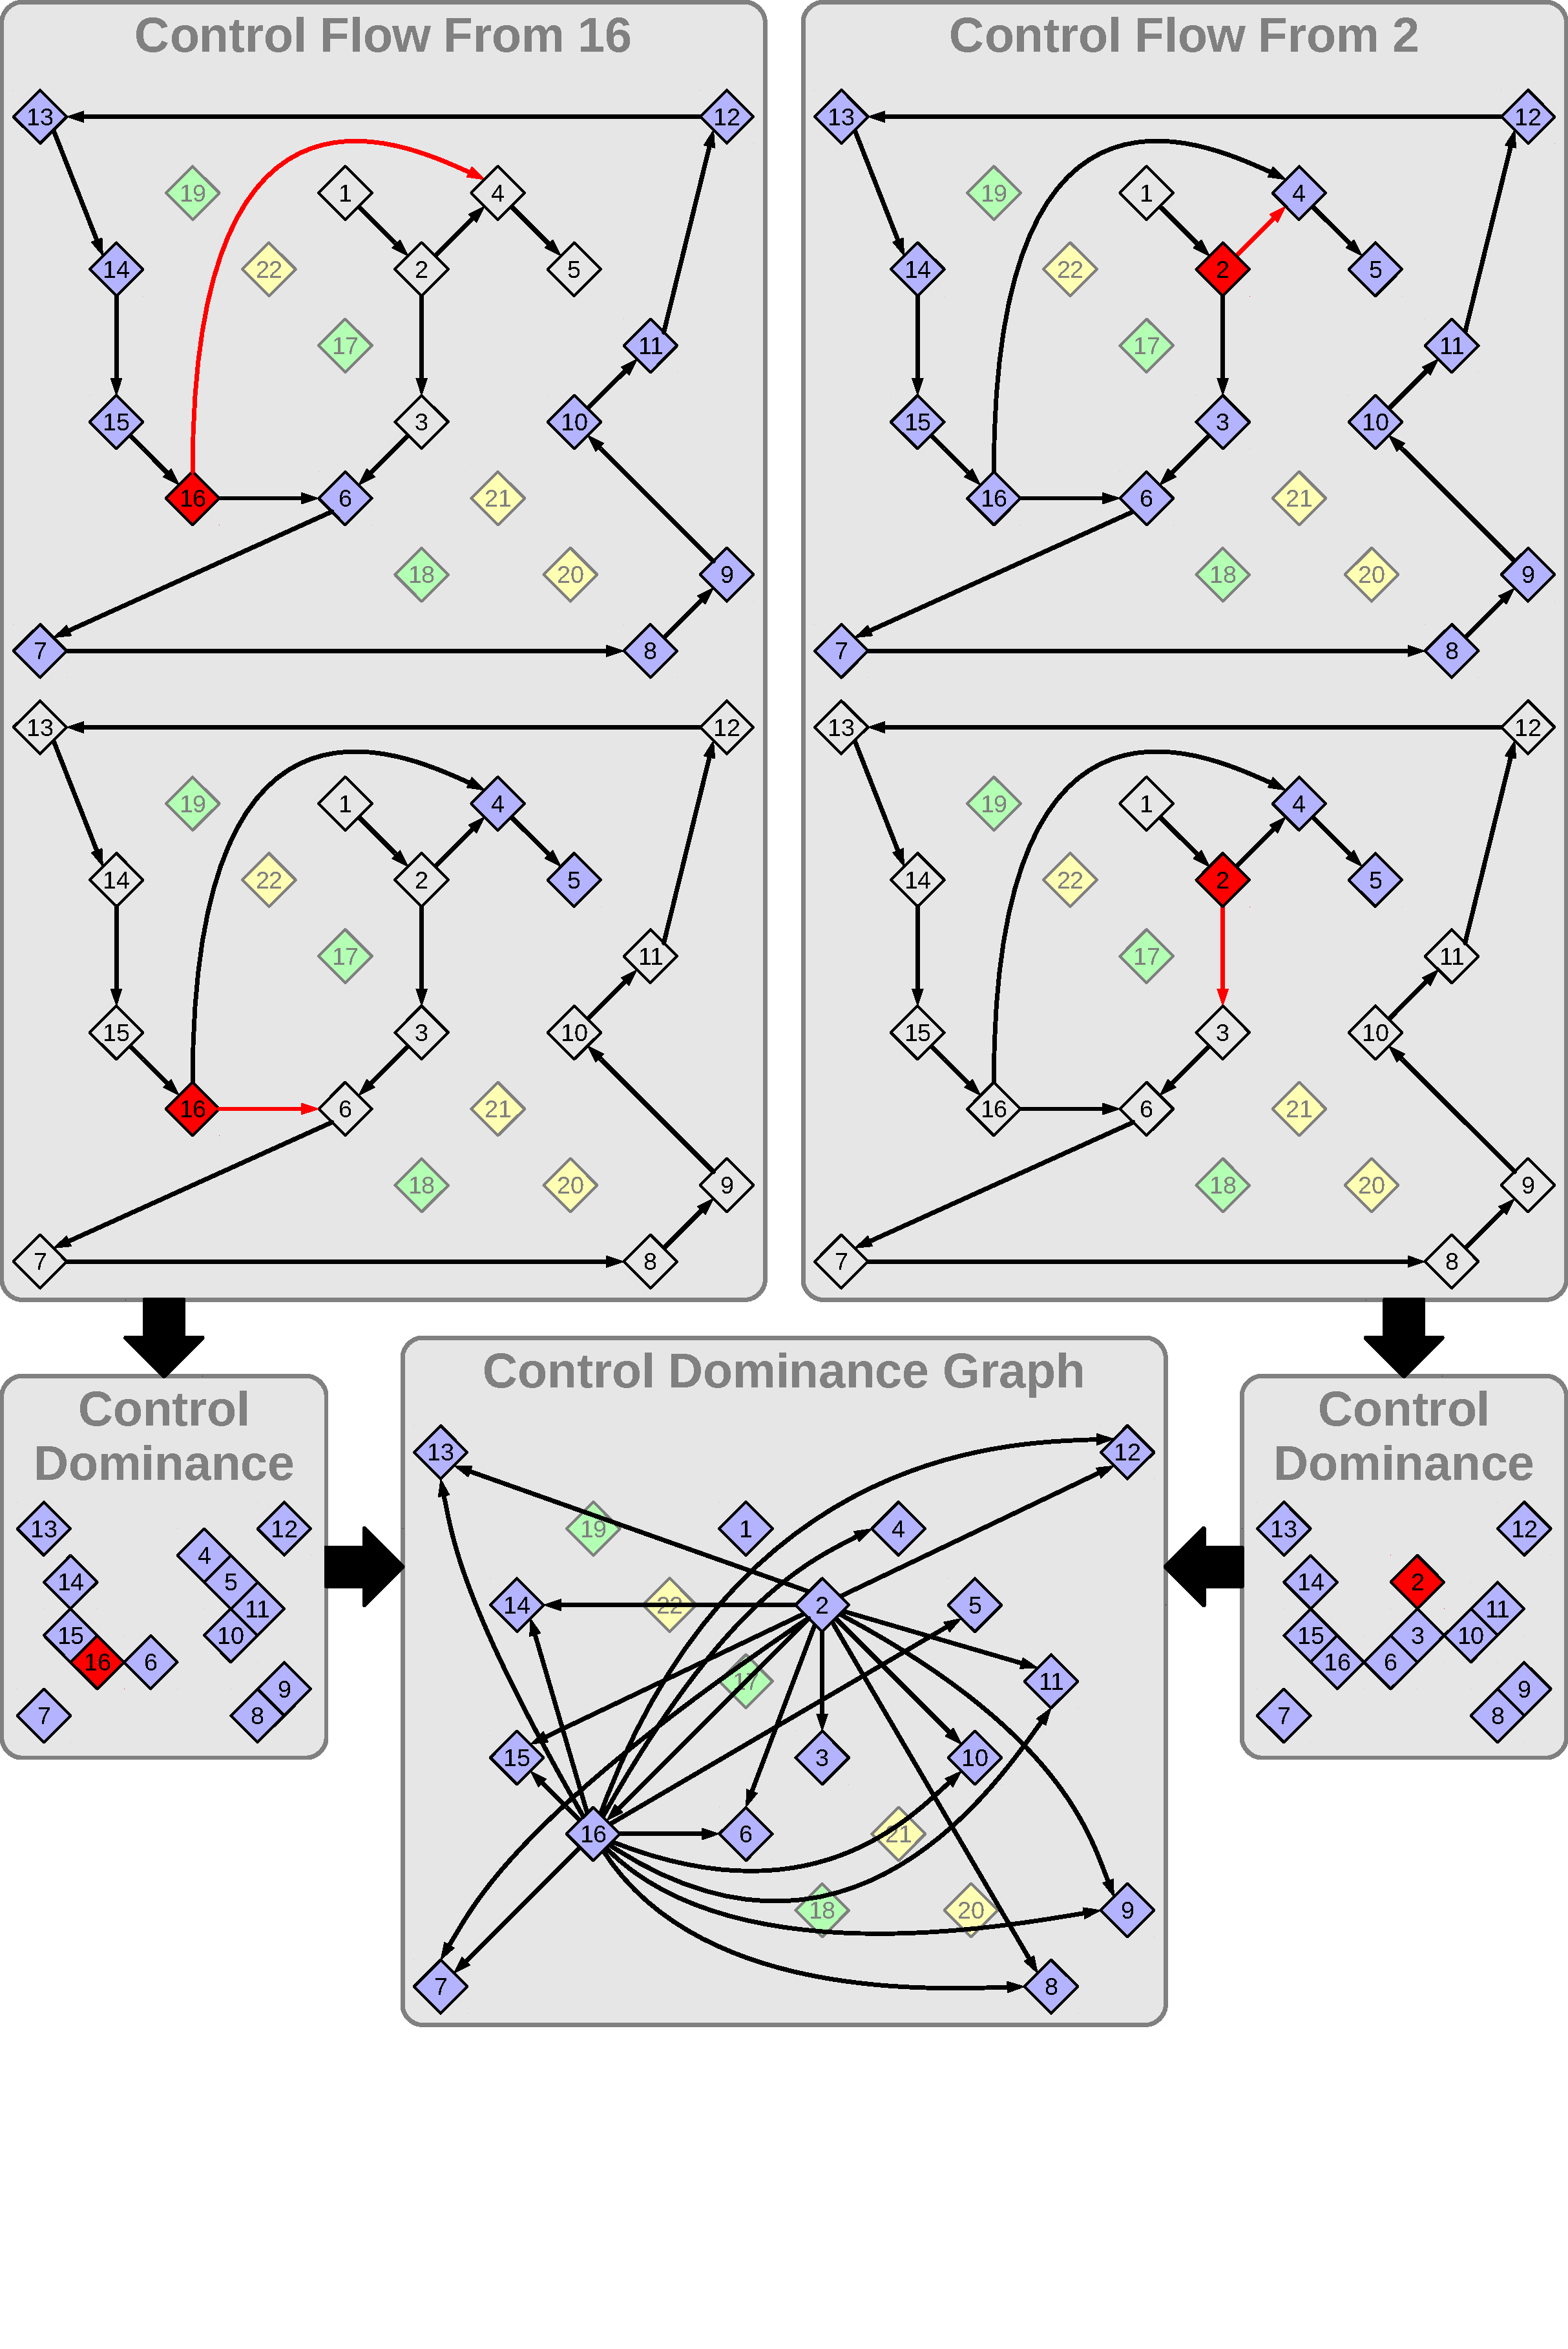
\includegraphics[width=\textwidth,height=1.5\textwidth]{figures/schaubild2.pdf}
%
%    \vspace{27.38136pt}
%    \caption{Computation of the control dependence graph.}
%    \label{fig:pdg}
%\end{figure}
%
%\subsection{Control Dependence Example}
%
%    The control dependence graph is a function of the control flow graph, as is
%    directly apparent from \Cref{def:cdg}.
%    We can see how an example control dependence graph is computed in
%    \Cref{fig:pdg}, from the control flow graph of the \texttt{dot} function
%    in \Cref{fig:derivemaths}.
%    From the definition it is immediately obvious that we need to only consider
%    conditional branches as origins of control dependence.
%
%    We can consider the two conditional branches $2$ and $16$ independently.
%    On the right, we consider only $2$.
%    We check the defining property: On the top of the figure, all the
%    instructions that are not reachable from $2$ without the edge $(2,4)$ are in
%    grey.
%    Below this, all instructions not reachable from $2$ without $(2,3)$ are
%    grey.
%    We see that $4,5$ are always reachable and $1$ is never reachable, these are
%    therefore not control dependent on $2$.
%    All the other instructions are control dependent on $2$.
%
%    Once we have computed this for all conditional branches, we take the union
%    on graphs and get the complete control dependence graph of the function.
%    Note what this graph represents:
%    Once the loop in the function has been unrolled, it contains a conditional
%    and a loop.
%    Eveything within the body of the conditional is control dependent on $2$.
%    Everythig within the loop as well as everything afterwards is control
%    dependent on $16$.
%
%\subsection{Phi Dependence Graph}
%
%    Phi nodes are fundamental in single static assignment form and need special
%    care.
%    The value that a phi node takes depends on from where a phi node was
%    reached.
%    We need to encapsulate this in a graph.
%
%    \begin{definition}{Phi Dependence Graph}{def:pog}
%        Let $p$ a phi node and $c$ a conditional branch instruction.
%        We say that the outcome of $p$ depends on $c$ if there is a branch
%        instruction $b$ that reaches $p$ such that $b$ is control dependent on
%        $c$.
%
%        This defines the {\em phi dependence graph} $\Phi DG_\mathcal{F}$.
%    \end{definition}
%
%
%\subsection{Program Dependence Graph}
%
%    After the control flow, data flow and control dependence graph, we lastly
%    introduce the {\em program dependence graph}.
%    It is the most exhaustive tool that we have to describe how values depend on
%    each other.
%
%    \begin{definition}{Program Dependence Graph}{def:pdg}
%        The {\em program dependence graph} is defined as the union of data flow
%        and control dependence graphs.
%        \begin{align*}
%            PDG_\mathcal{F}:=DFG_\mathcal{F}^*\cup CDG_\mathcal{F}^*\cup\Phi DG_\mathcal{F}\text{.}
%        \end{align*}
%    \end{definition}
%
%    With the program dependence graph, we can now define subsections of the
%    program that are self-contained and can be separated into their own
%    function.
%    This works even if they contain complicated control flow.
%    Firstly, we need a definition of an interface.
%
%    \begin{definition}{Interface}{def:interface}
%        Let $a\in CFG_\mathcal{F}^*$ and $b_1,\dots,b_n\in DFG_\mathcal{F}^*$.
%        Furthermore let $A\subset\mathbb{N}$ a set of instructions.
%
%        We say that $(b_1,\dots,b_n)$ is an interface to $A$ if it is a cut
%        between $o$ and $A$ in $PDG_\mathcal{F}$ for any of the following $o$:
%        \begin{itemize}
%            \item $o$ is a paramter
%            \item $o$ is impure
%        \end{itemize}
%    \end{definition}
%